%%%%%%%%%%%%%%%%%%%%%%%%%%%%%%%%%%%%%%%%%%
% Mathematics Final Year Research Projects
% LaTeX Template
% Version 1.0 (31/01/24)
%
% This template has been adapted from: https://www.overleaf.com/latex/templates/imperial-college-report-template/wncnzptkhnbc
% Students should feel free to adapt this template to their needs.
%%%%%%%%%%%%%%%%%%%%%%%%%%%%%%%%%%%%%%%%%%
%----------------------------------------------------------------------------------------
% PACKAGES AND OTHER DOCUMENT CONFIGURATIONS
%----------------------------------------------------------------------------------------
\documentclass[a4paper,11pt, twoside]{report}

%% Language and font encodings
\usepackage[english]{babel}
\usepackage[utf8]{inputenc}
\usepackage[T1]{fontenc}

%% Sets page size and margins
\usepackage[a4paper,top=1in,bottom=1in,left=1in,right=1in,marginparwidth=1.75cm]{geometry}

%% Useful packages
\usepackage{afterpage}
\usepackage{amsmath}
\usepackage{amsthm}
\usepackage{amssymb}
\usepackage{csquotes}
\usepackage{enumitem}
\usepackage{graphicx}
\usepackage{lipsum}
\usepackage{booktabs}
\usepackage{import} 
\usepackage{float} 
\usepackage{placeins}

\usepackage{subcaption}
\captionsetup[subfigure]{skip=8pt}
\captionsetup{skip=10pt}

\usepackage{xcolor}
\definecolor{oiOrange}{HTML}{E69F00}
\definecolor{oiTeal}{HTML}{009E73}

\usepackage{tikz}
\usepackage{tikz-3dplot}
\usepackage{tikz-3dplot-circleofsphere}
\usepackage{pgfplots}
\usepgfplotslibrary{groupplots}
\pgfplotsset{compat=1.18}
\usetikzlibrary{backgrounds,fillbetween}
\usepackage[utf8]{inputenc}

\usetikzlibrary{calc, intersections}
\usetikzlibrary{arrows.meta}
\tikzset{
    labelbg/.style={fill=white,inner sep=1pt,outer sep=0pt,rounded corners=1pt},
    dot/.style={circle,fill=black,inner sep=1.2pt},
    alphaArc/.style={draw=oiOrange, line width=1pt,{Stealth[length=2.4mm]}-},
    betaArc/.style ={draw=oiTeal,   line width=1pt,{Stealth[length=2.4mm]}-}
}
\usetikzlibrary{shapes.misc}

% Listings (for displaying code):
\usepackage{listings}
\lstset{
    frame = single, 
    framexleftmargin=15pt
}

\theoremstyle{definition}  % <-- 'definition' has upright text
\newtheorem{definition}{Definition}[chapter]
\newtheorem{remark}{Remark}[chapter]
\newtheorem{example}{Example}[chapter]
\newtheorem{lemma}{Lemma}[chapter]
\newtheorem{theorem}{Theorem}[chapter]
\newtheorem{corollary}{Corollary}[chapter]
\newtheorem{properties}{Properties}[chapter]
\newtheorem{proposition}{Proposition}[chapter]
\newtheorem{conjecture}{Conjecture}[chapter]



% Center figure captions:
\usepackage{caption}
\captionsetup[figure]{labelfont={bf},name={Figure},labelsep=quad}
\captionsetup[table]{labelfont={bf},name={Table},labelsep=quad}


% ----------- Algorithm2e setup
\usepackage[ruled,vlined]{algorithm2e}
\makeatletter
\renewcommand{\SetKwInOut}[2]{%
  \sbox\algocf@inoutbox{\KwSty{#2}\algocf@typo:}%
  \expandafter\ifx\csname InOutSizeDefined\endcsname\relax% if first time used
    \newcommand\InOutSizeDefined{}\setlength{\inoutsize}{\wd\algocf@inoutbox}%
    \sbox\algocf@inoutbox{\parbox[t]{\inoutsize}{\KwSty{#2}\algocf@typo:\hfill}~}\setlength{\inoutindent}{\wd\algocf@inoutbox}%
  \else% else keep the larger dimension
    \ifdim\wd\algocf@inoutbox>\inoutsize%
    \setlength{\inoutsize}{\wd\algocf@inoutbox}%
    \sbox\algocf@inoutbox{\parbox[t]{\inoutsize}{\KwSty{#2}\algocf@typo:\hfill}~}\setlength{\inoutindent}{\wd\algocf@inoutbox}%
    \fi%
  \fi% the dimension of the box is now defined.
  \algocf@newcommand{#1}[1]{%
    \ifthenelse{\boolean{algocf@inoutnumbered}}{\relax}{\everypar={\relax}}%
%     {\let\\\algocf@newinout\hangindent=\wd\algocf@inoutbox\hangafter=1\parbox[t]{\inoutsize}{\KwSty{#2}\algocf@typo\hfill:}~##1\par}%
    {\let\\\algocf@newinout\hangindent=\inoutindent\hangafter=1\parbox[t]{\inoutsize}{\KwSty{#2}\algocf@typo:\hfill}~##1\par}%
    \algocf@linesnumbered% reset the numbering of the lines
  }}%
\makeatother
% --------- end algorithm2e setup

% \bm allows typing bold math:
\usepackage{bm}
\usepackage[normalem]{ulem}

\usepackage[colorinlistoftodos]{todonotes}
\usepackage[colorlinks=true, allcolors=blue]{hyperref}

\renewcommand*{\rmdefault}{bch}
\renewcommand*{\ttdefault}{lmtt}
\newcommand{\citationneeded}{\textcolor{red}{[citation-needed]}}

\DeclareMathOperator*{\argmin}{\arg\!\min}
\DeclareMathOperator*{\argmax}{\arg\!\max}

% Add bigger skip between paragraphs, makes reading easier:
\setlength{\parskip}{0.5em}

% Bibliography
\usepackage[numbers, comma, square, sort&compress]{natbib}
\bibliographystyle{abbrvunsrtnat.bst}

%----------------------------------------------------------------------------------------
% END OF DOCUMENT CONFIGURATION
%----------------------------------------------------------------------------------------

%----------------------------------------------------------------------------------------
% IMPORTANT INFORMATION TO MODIFY FOR THE TITLE PAGE
%----------------------------------------------------------------------------------------
\newcommand{\reporttitle}{Min--Max Methods for Computing Planar Widths and Connections to the Allen--Cahn PDE} % Title of your research project
\newcommand{\reportauthor}{Siddharth Roshan Berera} % First Name and Last Name
\newcommand{\reportcid}{01858742} % First Name and Last Name
\newcommand{\reportyr}{2024-2025} % First Name and Last Name
\newcommand{\supervisor}{Professor M. A. M. Guaraco} % First Name and Last Name of your supervisor(s)
\newcommand{\degreetype}{MSc in Pure Mathematics} % MSci in Mathematics, BSc in Mathematics, BSc in Mathematics with Statistics, ...
%----------------------------------------------------------------------------------------

%----------------------------------------------------------------------------------------
% To compile this file, use the following sequence: 
%	latex main.tex
%	bibtex main.tex
%	latex main.tex
%	latex main.tex
%----------------------------------------------------------------------------------------

%----------------------------------------------------------------------------------------
% START OF DOCUMENT
%----------------------------------------------------------------------------------------
\setlength {\marginparwidth }{2cm} 
\begin{document}

% Title page
\begin{titlepage}

\newcommand{\HRule}{\rule{\linewidth}{0.5mm}} % Defines a new command for the horizontal lines, change thickness here

%----------------------------------------------------------------------------------------
%	LOGO SECTION
%----------------------------------------------------------------------------------------


\includegraphics[width=8cm]{title/logo.png}\\[1cm] % Include a department/university logo - this will require the graphicx package
 
%----------------------------------------------------------------------------------------

\center % Center everything on the page

%----------------------------------------------------------------------------------------
%	HEADING SECTIONS
%----------------------------------------------------------------------------------------

% For M3R or M4R reports, comment out as appropriate
\textsc{\LARGE Imperial College London}\\[0.5cm] % Name of your university/college
\textsc{\Large Department of Mathematics}\\[1.5cm] % Name of your department
\textsc{\Large MSc Research Project}\\[0.5cm] % Name of your programme
%\textsc{\LARGE BSc Research Project}\\[1.5cm] 

%----------------------------------------------------------------------------------------
%	TITLE SECTION
%----------------------------------------------------------------------------------------
\makeatletter
\HRule \\[0.6cm]
{ \huge \bfseries \reporttitle}\\[0.6cm] % Title of your document
\HRule \\[1.5cm]
 
%----------------------------------------------------------------------------------------
%	AUTHOR SECTION
%----------------------------------------------------------------------------------------

\begin{minipage}{0.4\textwidth}
\begin{flushleft} \large
\emph{Author:}\\
\reportauthor \\ % Your name
\emph{CID: }
\reportcid \\% Your name
\emph{Academic year: }
\reportyr% Your name
\end{flushleft}
\end{minipage}
~
\begin{minipage}{0.4\textwidth}
\begin{flushright} \large
\emph{Supervisor:} \\
\supervisor % Supervisor's name
\end{flushright}
\end{minipage}\\[2cm]
\makeatother

%----------------------------------------------------------------------------------------
%	FOOTER & DATE SECTION
%----------------------------------------------------------------------------------------
\vfill % Fill the rest of the page with whitespace
Submitted in partial fulfillment of the requirements for the \degreetype~at Imperial College London\\[0.5cm]

\makeatletter
{\large \today}\\[2cm] % Date, change the \today to a set date if you want to be precise
\makeatother

\end{titlepage}

% Abstract
\begin{abstract}
This dissertation develops a unified min--max framework connecting linear spectral theory, geometric widths and nonlinear PDEs. For linear operators, we construct spectra via a min--max scheme and show that the resulting critical points are determined by the topology of the underlying configuration space, yielding a form of topological invariance for min--max levels. In geometry, we formalise widths as nonlinear analogues of eigenvalues for length/area/volume functionals and prove that, for any convex polygon, the first width - an analogue of the second eigenvalue - equals the minimal supporting-line distance; the proof uses a novel and flexible topological argument that suggests extensions to broader width problems. Analytically, we realise widths as level sets of min--max solutions to the Allen--Cahn equation and implement a finite element scheme that computes nontrivial critical points. Together, these results show that min--max methods furnish a common framework for identifying fundamental invariants across linear, geometric and analytic settings, and that this framework is effective in computation.
\end{abstract}
 
% Acknowledgements
\clearpage
\section*{Acknowledgments}
\noindent I am deeply grateful to Professor M.\ A.\ M.\ Guaraco for his guidance, ideas, and encouragement throughout this project. I also thank my parents for their constant support and for patiently listening to countless discussions of my ideas.
\clearpage

% Acknowledgements
\clearpage
\section*{Plagiarism statement}
The work contained in this thesis is my own work unless otherwise stated. \\

\vspace{1em}
\noindent \textit{Signature:} \reportauthor \\
\textit{Date:} \today
\clearpage

% Table of contents
\tableofcontents

% Main sections of the report
% ===========================
% Uncomment or add folders to add your own chapters and input files.

\chapter{Introduction}
The \emph{min--max principle} is a unifying theme across analysis, geometry, and topology. At its core, it provides a strategy for identifying critical values of a functional by working not with single points, but with continuous families of points. One begins with a \textbf{space of objects} (often a function space), chooses a $p$-parameter \textbf{admissible family} of objects (typically forming a continuous submanifold of the space), evaluates a \textbf{functional} along this family, and records the unavoidable peak value - the \textbf{mountain to be crossed}. This is the essence of the \emph{mountain--pass algorithm}.  

The simplest case is $p=1$: a single path through the space. One can imagine the path as a string of balls connected by a thread, draped across a valley. Under gradient descent, each ball rolls downhill, but because they are tied together, some fall to one side, some to the other and at least one remains suspended at the saddle point across the valley floor. That ball marks a critical point of the functional. In higher dimensions, the same idea applies with $p$-parameter families: the greater the dimensionality of the family, the higher the ``mountain'' it is forced to cross. 

This perspective appears in many guises. In linear algebra, it underlies the variational characterisation of the eigenvalues of real symmetric matrices. In geometry, min--max methods are central to the construction of closed geodesics (Birkhoff \cite{Birkhoff27}) and minimal hypersurfaces (Almgren \cite{Almgren62}, Pitts \cite{Pitts81}, Marques--Neves \cite{MarquesNeves14}, \cite{MarquesNeves17}). In the study of nonlinear PDEs, mountain--pass arguments provide existence results for critical points of variational functionals (Guaraco \cite{Guaraco18}), such as the Allen--Cahn energy (Gaspar--Guaraco \cite{Guaraco16}).  

Although these applications are often studied in isolation, they share a unifying intuition: any continuous deformation within a constrained space must inevitably pass through certain “bottlenecks,” and these bottlenecks encode fundamental invariants of the system. This dissertation develops this theme in three domains of decreasing familiarity in the literature: first, the classical setting of linear spectral theory; second, the more recent framework of planar widths (Guth \cite{Guth07}); and third, the variational study of PDEs such as the Allen--Cahn equation.

 
\section{Overview and Key Results}
In Chapter \ref{ch:2}, we reinterpret the spectral theorem for real symmetric matrices through the min--max lens. In this case, the elements of the mountain--pass algorithm are the following: the \textbf{points in the space} are vectors in $\mathbb{R}^n$; the \textbf{admissible families} are $p$-dimensional linear subspaces intersected with the unit sphere; the \textbf{functional} is the \emph{Rayleigh quotient}, defined on $S^{n-1}\subset\mathbb{R}^n$; and the \textbf{mountains to be crossed} are the successive eigenvalues. The first eigenvalue arises simply by minimising the Rayleigh quotient over $S^{n-1}$. The second eigenvalue, however, cannot be obtained by direct minimisation; instead, it is characterised by taking all two-dimensional linear subspaces (whose intersections with $S^{n-1}$ are great circles), computing the maximum Rayleigh quotient along each, and then minimising over all such families. Higher eigenvalues are obtained analogously by considering $p$-dimensional subspaces, taking the maximum of the Rayleigh quotient over their intersections with $S^{n-1}$, and minimising over all such choices. This is summarised by the following theorem:
\begin{quote}
\textbf{Theorem \ref{CourantFischer} (Courant--Fischer Min--Max - linear setting).}  For a real symmetric matrix $A \in \mathbb{R}^{n \times n}$ with ordered eigenvalues $\lambda_1 \leq \cdots \leq \lambda_n$, the $k^{\text{th}}$ eigenvalue admits the min--max characterisation: $$\lambda_k=\min_{\substack{L\subset \mathbb{R}^n\\ \dim L = k}} \max_{\substack{\vec{v}\in L\\ \vec{v}\neq 0}} R(\vec{v}),$$
where $R:\mathbb{R}^n\setminus\{0\}\to \mathbb{R}$ is the Rayleigh quotient, $R(\vec v)=\dfrac{\langle \vec {v}, A\vec{v}\rangle}{\langle\vec v,\vec v\rangle}$.
\end{quote}
This is the linear prototype of the mountain--pass principle: eigenvalues arise as a progression of successive “mountain--passes,”  each forced by the dimensionality of the admissible families.\\
Building on this, we turn to \emph{homology} as a more flexible framework for organising admissible families in nonlinear settings. Linear subspaces tell directions apart using orthogonality, homology tells loops apart by how they \emph{wind}. Two closed curves are the same in homology if one can be slid into the other without cutting. On a torus there are two basic ways to go around (meridian and longitude), so any closed curve is determined, up to such sliding, by two integers \((m,n)\) counting how many times it winds in each direction. More compactly, \(H_1(T^2)\cong \mathbb{Z}\oplus\mathbb{Z}\). Replacing the linear subspaces in Courant--Fischer by homological cycles, we index admissible families by nontrivial classes in $H_p$. We now obtain min--max values because a nonzero class cannot be contracted to the trivial one within the admissible category.

\noindent \emph{Morse theory} refines this picture, relating the topology of the underlying space (say, the sphere carrying the Rayleigh quotient) to the number and indices of critical points: 
\begin{quote}
\textbf{Theorem \ref{MorseIneq} (Weak Morse Inequality).}
Let $M$ be a compact manifold and let $f:M\rightarrow R$ be a Morse function. Denote by $c_k \in \mathbb{N}$ the number of critical points of $f$ with index $k$, on $M$. Then
$$\beta_k(M) \leq c_k,$$
where $\beta_k(M) := \dim H_p(M;\mathbb{Z}_2)$ is the $k^{\text{th}}$ \emph{Betti} number of $M$. These inequalities show that nontrivial homology classes force the existence of critical points at the corresponding indices.
\end{quote}
In this sense, homological cycles replace linear subspaces, giving independent “directions of deformation” that produce robust mountain--pass levels. This perspective suggests running min--max over homology classes, giving a broad nonlinear analogue of the spectral framework.

\noindent Chapter \ref{ch:3} develops the geometric analogue via the notion of $p$-\emph{widths}, a nonlinear spectrum built using the min--max algorithm over families called sweep--outs. We focus on the \emph{first width} $(p=1)$ for planar domains. Informally, the simplest $1$-parameter sweep--out on the disc is given by a family of parallel chords. We use the horizontal chords out of convenience. 
\begin{figure}[ht]
  \centering
  \begin{tikzpicture}[line cap=round]
    \tikzset{pole/.style={circle, fill=black, inner sep=0pt, minimum size=2.2pt}}
  % parameters
  \def\R{2.4}      % radius (cm)
  \def\N{5}        % number of chords

  % compute spacing so chords don't sit on the boundary
  \pgfmathsetmacro{\step}{2*\R/(\N+1)}

  % draw chords inside the circle
  \begin{scope}
    \clip (0,0) circle (\R);
    \foreach \i in {1,...,\N} {
      \draw (-\R-0.3, -\R + \i*\step) -- (\R+0.3, -\R + \i*\step);
    }
  \end{scope}

  % circle outline last so it sits on top
  \draw (0,0) circle (\R);

  \node[pole, label={above:$t=1$}]   at (0,\R)   {};
  \node[pole, label={below:$t=-1$}]  at (0,-\R)  {};
\end{tikzpicture}

  \caption{Reference sweep--out by horizontal chords $\{\gamma_t^*\}_{t\in[-1,1]}$.}
\end{figure}
\FloatBarrier

\noindent For general disc--like domains, such as convex polygons, we understand a sweep--out as a continuous deformation of such a family. To make sweep-outs topologically nontrivial, we impose the condition that the map at the boundary has winding number 1. 
\begin{figure}[ht]
  \centering
  \begin{tikzpicture}[line cap=round]
  % parameters
  \def\R{2.6}   % disk radius
  \def\N{7}     % number of chords
  \def\t{1.0}   % 0 = straight chords, 1 = fully deformed
  \def\A{0.38}  % deformation amplitude (relative to R)

  % spacing of the reference chords
  \pgfmathsetmacro{\step}{2*\R/(\N+1)}

  % a smooth x-only warp (so ordering in y is preserved => no crossings)
  \pgfmathdeclarefunction{warp}{1}{%
    % argument is x/R (dimensionless). trig in radians -> add 'r'
    \pgfmathparse{0.35*sin(2*pi*#1 r) + 0.22*sin(5*pi*#1 r + 0.7) + 0.12*sin(9*pi*#1 r - 0.4)}%
  }

  \begin{scope}
    \clip (0,0) circle (\R);
    \foreach \i in {2,3,4,5,6} {
      \pgfmathsetmacro{\c}{-\R + \i*\step} % reference y-level
      \draw plot [smooth, samples=220, domain=-\R:\R]
        (\x, { \c + \t * \A * \R * warp(\x/\R) + 0.2*(\i-4)});
    }
  \end{scope}

  % boundary last
  \draw (0,0) circle (\R);
\end{tikzpicture}

  \caption{General sweep--out $\{\gamma_t\}_{t\in[-1,1]}$ on the disc .}
\end{figure}
\FloatBarrier

\noindent With this picture in mind, the first width is
\begin{equation}
    \omega_1(\Omega)=\inf_{(\{\gamma_t\})}\ \sup_{t\in[-1,1]}\mathrm{Length}(\gamma_t),   
\end{equation}

the least possible largest length among such sweep--outs. In this case, the elements of the mountain--pass framework are the following: the \textbf{points in the space} are submanifolds of a fixed domain; the \textbf{admissible families} are $1$-parameter \emph{sweep--outs} whose union covers the domain; the \textbf{functional} is the length of curves in the sweep--out; and the \textbf{mountain to be crossed} is the first width. Courant--Fischer characterises the second eigenvalue as follows: for each $2$-dimensional linear subspace $L\subset\mathbb{R}^n$ (so $L\cap S^{n-1}$ is a great circle), take the maximum of the Rayleigh quotient on $L\cap S^{n-1}$; then minimise this maximum over all such $L$. The first width is the analogous nonlinear construction: for each $1$-parameter family of curves (a sweep–out), take the maximum length occurring in the family; then minimise this maximum over all sweep–outs. In this sense $\{\omega_p\}$ acts as a nonlinear spectrum with $\omega_1$ playing the role of a “second eigenvalue” for the length functional. In this section we present a \textbf{novel proof}, based on a topological argument, of the first width of convex polygons: 
\begin{quote}
\textbf{Theorem \ref{thm:first-width-convex-polygon} (First width of convex polygons).}
Let $P\subset\mathbb{R}^2$ be a compact convex $n$-gon with edges $E_1,\dots,E_n$ and vertices $V_1,\dots,V_n$ labelled clockwise, cyclically. The first width equals the minimal distance between two parallel supporting lines of $P$:
\[
\omega_1(P)
= \min_{\|\vec{u}\|=1} \big( \max_{\vec{x}\in P} \vec{x}\!\cdot \vec{u} - \min_{\vec{x}\in P} \vec{x}\!\cdot \vec{u} \big)
= \begin{cases}
        \displaystyle \min_{1\le i\le n}\ \operatorname{dist}\!\big(V_i,E_{V_i}^{\mathrm{opp}}\big), & \text{if $n$ is odd},\\
        \displaystyle \min_{1\le i\le n}\ \operatorname{dist}\!\big(E_i,E_{E_i}^{\mathrm{opp}}\big), & \text{if $n$ is even}.
    \end{cases}
\]
Here $E_{V_i}^{\mathrm{opp}}$ denotes the unique edge opposite the vertex $V_i$ when $n$ is odd, and $E_{E_i}^{\mathrm{opp}}$ denotes the unique 
edge opposite $E_i$ when $n$ is even. For a triangle this reduces to “$\omega_1 =$ smallest altitude.”
\end{quote}
While the equality itself is known in the literature (see \cite{Chodosh25}), our contribution is providing a \emph{new proof} that the minimal distance between opposite supports is a lower bound for the first width. The main idea in our method, which can be found in Lemma (\ref{lem:polygon-width-ub}), is to track endpoints of the curves throughout the sweep--out, view their evolution as a loop on the torus, and designate a target set on the torus (another loop) that realises the claimed width. By known results on the intersection number of loops on $T^2$, the endpoint loop meets this target set, forcing a curve of length at least the claimed value (lower bound). A matching upper bound comes from a parallel--line sweep--out that attains this distance. This viewpoint is flexible and suggests extensions to other sweep--out and width problems, which we discuss in the Further Directions, Chapter \ref{ch:5}.

\noindent Finally in Chapter~\ref{ch:4}, we consider a third problem in the mountain--pass setting. In this case, the elements of the mountain--pass algorithm are as follows. The \textbf{points} are functions in an appropriate Hilbert space. The \textbf{admissible families} are smooth $p$-parameter families in that space. The \textbf{functional} is the \emph{Allen--Cahn energy}
\[
E_\varepsilon(u)=\int_{\Omega} \frac{\varepsilon}{2}\,|\nabla u|^2+\frac{1}{\varepsilon}W(u),
\]
whose Euler--Lagrange equation is the Allen--Cahn PDE
\[
-\varepsilon\,\Delta u+\frac{1}{\varepsilon}\,W'(u)=0 \quad \text{in } \Omega.
\]
The \textbf{mountains} are the nontrivial critical values of this energy obtained via such families.Concretely, fix a smooth double--well potential $W$ and let $c_\varepsilon$ denote the associated min--max critical level. Guaraco showed that, after the natural Modica--Mortola rescaling,
\[
\frac{1}{2\sigma}\,c_\varepsilon\ \longrightarrow\ \omega_1(\Omega)\qquad(\varepsilon\to 0),
\qquad
\sigma=\int_{-1}^{1}\sqrt{2W(s)}\,ds,
\]
thereby providing a PDE realisation of geometric widths and a route to minimal hypersurfaces via Allen--Cahn. Geometrically, the min--max solution $u_\varepsilon$ develops a thin transition layer where $u_\varepsilon$ crosses between the wells; as $\varepsilon\to 0$ the level sets (e.g. $\{u_\varepsilon=0\}$) concentrate on a rectifiable curve $\Gamma\subset\Omega$ that is stationary for length and satisfies $\mathrm{Length}(\Gamma)=\omega_1(\Omega)$. In other words, the Allen--Cahn interfaces ‘draw’ the width–realising curve in the small–$\varepsilon$ limit, with $E_\varepsilon(u_\varepsilon)/(2\sigma)\to \mathrm{Length}(\Gamma)=\omega_1(\Omega)$.

Our focus here is twofold: \emph{theoretically}, we make this correspondence precise by discussing that transition layers of min--max Allen--Cahn solutions converge, as $\varepsilon\to 0$, to curves realising the widths of $\Omega$; and \emph{computationally}, we complement this with two numerical implementations of the mountain--pass principle—(i) for the area functional, discretising a cylindrical domain by a triangular mesh and running a mountain--pass algorithm on the area viewed as a function of vertex positions, thereby obtaining discrete saddle--type critical points such as the catenoid; and (ii) for the Allen--Cahn energy, approximating the infinite--dimensional function space by a finite--element discretisation and computing nontrivial critical points via an analogous mountain--pass search. In parallel with Guaraco’s theorem—showing that Allen--Cahn min--max energies converge (after rescaling) to geometric widths—our computed min--max energies reflect these underlying geometric invariants. Taken together, these experiments demonstrate how the min--max framework can be made computational, linking discrete algorithms with the analytic and geometric theory.

\chapter{Min--Max Methods for Computing the Spectrum of Linear Operators}
\label{ch:2}
% ==========================================================
In this section we illustrate how min--max methods recover the spectrum of a linear operator, beginning with the classical case of real symmetric matrices. 
The linear setting serves as a prototype: here eigenvalues can be computed by standard algebraic means, but the min--max approach reveals a deeper structure that later extends to nonlinear operators, where no closed-form diagonalisation exists.\\
We recall the basic definitions. Let $A:\mathcal{H}\to\mathcal{H}$ be a linear operator on a Hilbert space $\mathcal{H}$ over a field $\mathbb{F}$.

\begin{definition}[Eigenvectors and Eigenvalues]\label{eigen}
A nonzero vector $\vec v \in \mathcal H$ is an \emph{eigenvector} of $A$ if there exists a scalar $\lambda \in \mathbb{F}$ such that 
\begin{align*}
A(\vec v) = \lambda \vec v.
\end{align*}
The scalar $\lambda$ is the corresponding \emph{eigenvalue}.
\end{definition}

\noindent To connect eigenvalues with a variational principle, we introduce the \emph{Rayleigh quotient}, a functional whose critical points are precisely eigenvectors. 

\begin{definition} [Rayleigh Quotient]
The Rayleigh Quotient associated with the linear operator $A$ is the function  
\begin{align*}
    R:\mathcal{H}\setminus\{0\}\to \mathbb{F}, \qquad
R(\vec v) = \frac{\langle A\vec v, \vec v\rangle}{\langle \vec v, \vec v\rangle}.
\end{align*}
If $\vec{v}$ is an eigenvector with eigenvalue $\lambda$, then $R(\vec{v})=\lambda$.
\end{definition}


\section{The Spectral Theorem and Min--Max over Linear Subspaces}
\noindent Specialising to $\mathcal{H} = \mathbb{R}^n$ with the standard inner product $\langle \cdot,\cdot\rangle$, we take $A:\mathbb{R}^n\to\mathbb{R}^n$ to be a real symmetric matrix. 
Observe that $R$ is homogeneous of degree zero: for any $a \neq 0$, $R(a\vec v) = R(\vec v)$. Thus $R$ naturally descends to the unit sphere $S^{n-1}$, being constant along rays through the origin.
Since $R(\vec v) = R(-\vec v)$, the quotient further descends from $S^{n-1}$ to real projective space $\mathbb{RP}^{n-1}$, the true natural domain of the Rayleigh quotient. We postpone the formal definition of $\mathbb{RP}^{n-1}$ until it is needed, but for now continue working with $S^{n-1}$.

\noindent In the mountain-pass analogy, the Rayleigh quotient plays the role of the landscape, with eigenvalues appearing as critical heights.

\noindent To make this framework precise, we must verify that the critical points of the Rayleigh quotient on $S^{n-1}$ coincide with the eigenvectors of $A$. This is the key step that connects the variational perspective with linear algebra, and it is formalised in the following lemma.

\begin{lemma} \label{RayleighCPs}
Let $A:\mathbb R^n \to \mathbb R^n$ be symmetric. A nonzero vector $\vec{v} \in \mathbb R^n$ is a critical point of the Rayleigh quotient $R$ if and only if $\vec{v}$ is an eigenvector of $A$, in which case $R(\vec{v})$ equals the corresponding eigenvalue.
\end{lemma}
\begin{proof}
Differentiating $R$ with respect to $\vec{v}$ gives
\begin{equation}\label{eq:RQgrad}
   \nabla_{v} R = \frac{2A\vec{v}\langle \vec{v}, \vec{v} \rangle - 2\vec{v}\langle A\vec{v}, \vec{v} \rangle}{\langle \vec{v}, \vec{v} \rangle^2}. 
\end{equation}
Setting the gradient to $\vec{0}$ and solving for the critical points,
\begin{align*}
\frac{2A\vec{v}\langle \vec{v}, \vec{v} \rangle - 2\vec{v}\langle A\vec{v}, \vec{v} \rangle}{\langle \vec{v}, \vec{v} \rangle^2} = \vec{0}, \\
\Leftrightarrow A\vec{v} = \frac{\langle A \vec{v},\vec{v}\rangle}{\langle \vec{v}, \vec{v} \rangle} \vec{v}, \\
\Leftrightarrow A\vec{v} = R(\vec{v})\vec{v}. \\
\end{align*}
By Definition (\ref{eigen}) of eigenvectors and eigenvalues, this has solutions for $\vec{v}$ which are precisely the eigenvectors of $A$ and with the value of $R$ being the corresponding eigenvalues.
\end{proof}

\noindent Thus the “mountains” are realised as critical levels of $R$. The landscape is further clarified by the relation between different peaks: eigenvectors associated with distinct eigenvalues do not tilt toward each other but instead lie in perpendicular directions. This orthogonality is formalised in the next lemma. 

\begin{lemma} \label{eigenvec_perp}
If $\vec{v}_i, \vec{v}_j \in \mathbb{R}^n$ ($i\neq j$) are eigenvectors of the symmetric matrix $A:\mathbb{R}^n\rightarrow\mathbb{R}^n$, with distinct eigenvalues $\lambda_i, \lambda_j \in \mathbb{R}$, respectively then $\vec{v}_i \perp \vec{v}_j$.
\end{lemma}
\begin{proof}
Since $\vec{v}_i, \vec{v}_j$ are eigenvectors with corresponding eigenvalues $\lambda_i, \lambda_j$ by definition (\ref{eigen}) we have that $A\vec{v}_i = \lambda_i \vec{v}_i$ and $A\vec{v}_j = \lambda_j \vec{v}_j$. Thus, 
\begin{align*}
\langle \lambda_i\vec{v}_i, \vec{v}_j \rangle = \langle A\vec{v}_i, \vec{v}_j \rangle &= \langle \vec{v}_i, A\vec{v}_j \rangle = \langle \vec{v}_i, \lambda_j\vec{v}_j \rangle, \\
\Rightarrow \lambda_i = \lambda_j \quad &\text{or} \quad \langle\vec{v}_i,\vec{v_j}\rangle = 0.
\end{align*}
Since $\lambda_i\neq \lambda_j$, we conclude that $\langle \vec{v}_i, \vec{v}_j \rangle = 0$.
\end{proof}

\noindent Orthogonality ensures that eigenvectors associated with distinct eigenvalues span mutually perpendicular directions. This orthogonal structure allows us to iteratively ‘peel away’ subspaces: once $k$ eigenvectors are known, minimising the Rayleigh quotient on their orthogonal complement reveals the next eigenvector. The following lemma makes this precise.

\begin{lemma} \label{lemma23}
Let $\vec{v}_1,\cdots, \vec{v}_k \in \mathbb{R}^n$, $k<n$, be a set of eigenvectors of the symmetric matrix $A:\mathbb{R}^n\rightarrow\mathbb{R}^n$ and denote by $L_k :=span\{\vec{v}_1,\cdots, \vec{v}_k\}$. The minimiser of the Rayleigh Quotient over the orthogonal complement $L_k^{\perp}$ is a new eigenvector.
\end{lemma}
\begin{proof}
To prove this, we restrict the Rayleigh quotient to the orthogonal complement of the first $k$ eigenvectors. The idea is that minimising on this smaller space yields a new critical point, and hence a new eigenvector. Let $$\mathcal{M}:=\{\vec{x}\in L_{k}^{\perp}:||\vec{x}||=1\},$$ be the submanifold of the domain of $R$, $S_{n-1}$, in the orthogonal complement. 

\begin{figure}
    \centering
    \def\r{3}
\tdplotsetmaincoords{70}{125}

\begin{tikzpicture}[tdplot_main_coords]
\path[use as bounding box] (-8,-15) rectangle (8,15);
  \begin{scope}[thin,black!30]

    \draw[->] (-1.8*\r,0,0) -- ( 2*\r,0,0)
          node[anchor=north east] {};

    \draw[->] (0,-1.5*\r,0) -- (0, 2*\r,0)
          node[anchor=north] {$L_k$};

    \draw[->] (0,0,-1.3*\r) -- (0,0, 1.5*\r)
          node[anchor=south east] {};

    % sphere outline in screen coords
    \draw[tdplot_screen_coords] (0,0,0) circle (\r);

    % latitude circle in coordinate system coords
    \tdplotCsDrawLatCircle{\r}{0}
    \node[gray,anchor=west] at (-1,3,1) {$S^{n-1}$};

  \end{scope}


  % a filled great circle slice (adjust angles / style as desired)
  \tdplotCsDrawGreatCircle[
      tdplotCsFill/.style={green,opacity=0.2}
  ]{\r}{-90}{100}
  \node[black,anchor=west] at (4.25,0,1) {$\mathcal{M}$};

  \draw[->,thick] (0,0,0) -- (1.8,0,3.2);
  \node[anchor=south east] at (1.8,0,3.2) {$\vec{u}$};


  \begin{scope}[thick,>=stealth]      % choose arrow‑tip style
%--- translucent tangent parallelogram spanned by e1, e2 ------------
  \fill[blue!30,opacity=0.4]   % colour & transparency -- change as desired
    ( 5.85,  4.08, 3.2) --
      ( 5.85, -0.72, 3.2) --
      (-1.44, -2.664,3.2) -- 
      (-1.44,  2.136,3.2) --
      cycle;

  \draw[black,very thin]
      ( 5.85,  4.08, 3.2) --
      ( 5.85, -0.72, 3.2) --
      (-1.44, -2.664,3.2) -- 
      (-1.44,  2.136,3.2) -- 
      cycle;

    % e1  (red)  0.3 units in +x direction
  \draw[->,blue]   (1.8,0,3.2) -- ++(6.1875,1.65,0)
        node[anchor=east] {$T_{\vec{u}}\mathcal{M}$};

  % e2  (blue) 0.3 units in +y direction
  \draw[->,red]  (1.8,0,3.2) -- ++(0,3.65,0)
        node[anchor=west, xshift=2pt,yshift=12pt] {$\langle \vec{v}_1,\cdots,\vec{v}_k\rangle$};

  % e3  (green) 0.3 units in +z direction
  \draw[->,violet] (1.8,0,3.2) -- ++(1.8,0,3.2)
        node[anchor=south east] {$\alpha \vec{u}$};
\end{scope}

  

\end{tikzpicture}

    \caption{The submanifold $\mathcal{M} = S^{n-1} \cap L_k^\perp$ (green, a great circle in this $3$--dimensional illustration) together with its orthogonal components.}
    \label{fig:placeholder}
\end{figure}
\FloatBarrier

\noindent Note firstly that since $k<n$, the orthogonal complement and thus $\mathcal{M}$ are not empty, and secondly that minimising $R$ on $\mathbb{R}^n\setminus\{\vec{0}\}$ is equivalent to minimising on the compact set $\mathcal{M}$ (by scale invariance). Define also the tangent space to $\mathcal{M}$ at $\vec{u}$, $$T_{\vec{u}}\mathcal{M} = \{ \vec{{w}\in L_k^{\perp} } : \langle \vec{w},\vec{u}\rangle = 0\}.$$ Since the map $R|_{\mathcal{M}}: \mathcal{M} \rightarrow \mathbb{R}$ is continuous it attains its minimum on $S$ at some unit vector $\vec{u}\in L_{k}^{\perp}$.  Let $$\lambda:=R(\vec{u}) = \min_{\vec{x}\in \mathcal{M}} R(\vec{x}).$$ We proceed to show that $\vec{u}$ is a critical point of $R$. \\

\textbf{Claim 1: $\nabla R(\vec{u}) \perp \vec{u}$.} \\
Since $R$ is scale invariant and thus constant along the ray through the origin, its directional derivative along $\vec{u}$ vanishes identically. \\

\textbf{Claim 2: $\nabla R(\vec{u}) \perp \mathcal{M}$.} \\
Since $\vec{u}$ is the minimiser of $R$ in $\mathcal{M}$, a smooth submanifold of $S^{n-1}$ with no boundary, it is a critical point of $R$ restricted to $\mathcal{M}$ and so its gradient projected onto any vector $\vec{w} \in T_{\vec{u}}\mathcal{M}$ is $0$. \\

\textbf{Claim 3: $\nabla R(\vec{u}) \perp L_k$.} \\
By Equation (\ref{eq:RQgrad}) for the gradient of the $R$ and noting that $||\vec{u}||=1$, we have for any of the $v_j$s the following, $$\langle \nabla R(\vec{u}), \vec{v}_j \rangle = \langle 2A\vec{u} - 2\vec{u}\langle A\vec{u}, \vec{u} \rangle, \vec{v}_j\rangle.$$ Since $\vec{u}\perp\vec{v}_j$ as they live in each others orthogonal complements, $$\langle \nabla R(\vec{u}), \vec{v}_j \rangle = \langle 2A\vec{u}, \vec{v}_j\rangle = 2\langle \vec{u}, A\vec{v}_j\rangle = 2\langle \vec{u}, \lambda_j\vec{v}_j\rangle,$$ which once again is zero as $\vec{u}$ and $\vec{v}_j$ are orthogonal to one and other. Thus $\langle \nabla R(\vec{u}), \vec{v}_j \rangle = 0$ for each $j \in \{1,\cdots,k\}$ and so $\langle \nabla R(\vec{u}), \vec{z} \rangle = 0$ for any $\vec{z} \in L_k$. \\

\noindent Finally, since $$\mathbb{R}^n = \text{span}\{\vec{u}\} \oplus T_{\vec{u}}\mathcal{M} \oplus L_k,$$

\noindent the gradient vanishes in every direction, so $\vec u$ is a genuine critical point of $R$ in the whole domain $S^{n-1}$ (not just in $\mathcal{M}$). By Lemma (\ref{RayleighCPs}) we have then that the minimiser of $R$ over $\mathcal{M}$, $\vec{u}$, is indeed an eigenvector of $A$ as claimed.
\end{proof}

\noindent In the mountain pass dictionary, this shows that restricting to orthogonal complements corresponds to seeking new ‘passes’ beyond the previously discovered peaks. Each minimisation step forces us onto a new mountain ridge, yielding a fresh eigenvalue. This completes the min–max step: having shown that minimising on orthogonal complements generates new eigenvectors, we are now ready to assemble these ingredients into the spectral theorem.

\begin{theorem}[Spectral theorem over $\mathbb R$]\label{SpectralThm}
Every real symmetric matrix $A\in\mathbb R^{n\times n}$ has an orthonormal basis of eigenvectors. Equivalently, there exist an orthogonal $Q$ and a real diagonal $D$ with $A=QDQ^{\top}$.
\end{theorem}
\begin{proof}
\textbf{Step 1: existence of at least one eigenvector.}
Consider the Rayleigh quotient, $R$ associated with $A$ on the unit sphere $S^{n-1}$.  Since $S^{n-1}$ is compact and $R$ is smooth on this domain, it attains a minimum (and a maximum) on $S^{n-1}$ at some $\vec{u}\in S^{n-1}$. Since minimising a smooth function on a smooth constraint set (the unit sphere), any global minimiser is a local minimiser and so a critical point of the function. By Lemma (\ref{RayleighCPs}), $\vec{u}$ is a critical point of $R$, hence an eigenvector of $A$.

\textbf{Step 2: induction.}
Let $\vec{v}_{1}$ be a unit eigenvector found in Step~1.  Suppose we have found $k<n$ \emph{orthonormal} eigenvectors $\vec{v}_{1},\dots,\vec{v}_{k}$ of $A$. Set $L_{k}=\operatorname{span}\{\vec{v}_{1},\dots,\vec{v}_{k}\}$ and consider its orthogonal complement $L_{k}^{\perp}$.  By Lemma (\ref{eigenvec_perp}) the $v_{j}$ are mutually orthogonal, so $\dim L_{k}^{\perp}=n-k\ge1$. Minimise $R$ on the compact set $S_{k}:=\{\vec{x}\in L_{k}^{\perp}:\|\vec{x}\|=1\}$, noting that by Lemma (\ref{lemma23}) a minimiser $\vec{v}_{k+1}$ exists and is an eigenvector of $A$ and, by construction, $\vec{v}_{k+1}\perp L_{k}$; normalise it to have unit length. By Lemma (\ref{eigenvec_perp}), $\vec{v}_{k+1}$ is orthogonal to each $\vec{v}_{j}$, $j\le k$. Thus we can extend the orthonormal eigenfamily by one vector.  Iterating, after $n$ steps (see remark \ref{rem:repeated-eigen}) we obtain orthonormal eigenvectors $\vec{v}_{1},\dots,\vec{v}_{n}$, which form an orthonormal basis of $\mathbb R^{n}$. Adding any more eigenvectors would not be possible as by Lemma (\ref{eigenvec_perp}) they must all be mutually orthogonal and at most $n$ vectors in $\mathbb{R}^n$ can satisfy this.

\textbf{Step 3: diagonalisation.}\label{step:diagonalisation}
Let $Q=[\vec{v}_{1}\ \cdots\ \vec{v}_{n}]$ (orthonormal) and $D=\operatorname{diag}(\lambda_{1},\dots,\lambda_{n})$ with $A\vec{v}_{j}=\lambda_{j}v_{j}$. Then $AQ=QD$, hence $A=QDQ^{\top}$.
\end{proof}
\begin{remark}\label{rem:repeated-eigen}
If an eigenvalue has multiplicity $m>1$, the procedure will return $m$ independent eigenvectors for it before proceeding to the next eigenvalue. These can be orthogonalised, so the construction still yields a total of $n$ orthonormal eigenvectors with the process having fewer iterations and more eigenvectors for some of those iterations.
\end{remark}


\subsection{From Courant--Fischer to the Mountain Pass Principle}
The inductive argument in Theorem (\ref{SpectralThm}) repeatedly applied the algorithm behind the proof of Lemma (\ref{lemma23}): given eigenvectors for the $k$ smallest eigenvalues, minimise the Rayleigh quotient in the orthogonal complement to discover the next one. This iterative algorithm can be summarised and sharpened in via the Courant--Fischer theorem.

\begin{theorem}[Courant--Fischer Min--Max \cite{Bhatia97}]\label{CourantFischer}
 Assume the eigenvalues of the real symmetric matrix $A$ are ordered $\lambda_1 \leq \cdots \leq \lambda_n$, with corresponding orthonormal eigenbasis $\{\vec{w}_1,\cdots,\vec{w}_n\}$. The eigenvalues of $A$ admit the following min-max characterisation: $$\lambda_k=\min_{\substack{L\subset \mathbb{R}^n\\ \dim L = k}} \max_{\substack{\vec{v}\in L\\ \vec{v}\neq 0}} R(\vec{v}).$$
\end{theorem}
\begin{proof}
Let $k \in \{ 1,..., n\}$ be fixed.

\textbf{Step 1: Upper Bound for $\lambda_k$.}
Pick the particular $k$-dimensional subspace $L_0=span\{\vec{w}_{1}\ \cdots\ \vec{w}_{k}\}$, then for $\vec{z} \in L_0$ we can write $\vec{x} = \sum_{i=1}^{k} \alpha_i \vec{w_i}$ and,
\begin{align*}
R(\vec{z}) = \frac{\langle A\vec{z}, \vec{z} \rangle}{\langle \vec{z}, \vec{z} \rangle} &= \frac{\langle \sum_{i=1}^k \alpha_i A\vec{w_i}, \sum_{i=1}^k \alpha_i\vec{w_i} \rangle}{\langle \sum_{i=1}^k \alpha_i\vec{w_i}, \sum_{i=1}^k \alpha_i\vec{w_i} \rangle} = \frac{\langle \sum_{i=1}^k \alpha_i \lambda_i\vec{w_i}, \sum_{i=1}^k \alpha_i\vec{w_i} \rangle}{\langle \sum_{i=1}^k \alpha_i\vec{w_i}, \sum_{i=1}^k \alpha_i\vec{w_i} \rangle}, \\
\Rightarrow R(\vec{z}) &= \frac{\sum_{i=1}^k\alpha_i^2 \lambda_i}{\sum_{i=1}^k \alpha_i^2} \leq \lambda_k.
\end{align*}
Thus $\max_{\vec{z}\in L_0} R(\vec{z}) \leq \lambda_k$ and so 
\begin{equation}\label{UpperBound}
\min_{\substack{\dim L = k}} \max_{\substack{\vec{v}\in L \\ \vec{v}\neq 0}} R(\vec{v}) \leq \lambda_k.
\end{equation}

\textbf{Step 2: Lower Bound for $\lambda_k$.}
Let $L$ be any $k$-dimensional subspace. Set $H:=span\{\vec{w}_k,\cdots,\vec{w}_n\}$ (dimension $n-k+1$).
By the dimension formula,
\[
dim(L\cap H) \geq dim(L) + dim(H) - n = k + (n-k+1) - n = 1,
\]
so there exists nonzero $\vec{z}\in L\cap H$. As $\vec{z}\in H$ we can write it as $\vec{z} = \sum_{i=k}^n \alpha_i \vec{w_i}$. Then, 
\[
R(\vec{z}) = \frac{\sum_{i=k}^n\alpha_i^2 \lambda_i}{\sum_{i=k}^n \alpha_i^2} \geq \lambda_k,
\]
so $\max_{\vec{v}\in L} R(\vec{v}) \geq  \lambda_k$ for any $k$-dimensional $L$. This implies that, 
\begin{equation}\label{LowerBound}
\min_{\substack{\dim L = k}} \max_{\substack{\vec{v}\in L \\ \vec{v}\neq 0}} R(\vec{v}) \geq \lambda_k.
\end{equation}
Finally, combining the inequalities (\ref{UpperBound}) and (\ref{LowerBound}), we have the desired equality.
\end{proof}

\noindent\textbf{Link to the mountain-pass picture.}
The Courant--Fischer theorem realises the mountain–pass analogy in exact algebraic form.  
\begin{itemize}
    \item The \textbf{space of points} is again the sphere $S^{n-1}$.  
    \item A $k$-dimensional subspace $L$ plays the role of a \textbf{$k$-parameter family}, a constrained region through which one must pass.  
    \item The \textbf{functional} is the Rayleigh quotient $R(\vec v)$.  
    \item The \textbf{mountains} are the eigenvalues: for any choice of $L$, one cannot avoid climbing to at least the level $\lambda_k$.  
\end{itemize}
Thus the $k$-th eigenvalue is exactly the critical height of the lowest unavoidable pass across all $k$-dimensional routes. This interpretation highlights why min–max methods, first glimpsed here in the linear setting, extend so naturally to nonlinear PDEs and variational problems.


\section{Homology as a Robust Alternative to Linear Subspaces}\label{section:cyclesboundaries}
So far, our min--max characterisations of eigenvalues (Theorems~\ref{SpectralThm} and \ref{CourantFischer}) have used $k$-dimensional \emph{linear} subspaces as test families, which is exactly right for the \emph{linear} setting. In the next chapter, however, we study \emph{nonlinear} functionals (e.g. length), where the configuration space lacks a natural linear test structure and linear subspaces are too rigid to enforce the global obstruction required for a nontrivial critical point. In that nonlinear settings, the appropriate notion of “$k$ degrees of freedom” is \emph{topological} rather than linear: one works with $k$-parameter sweep--outs (continuous families) organised by a nontrivial homology class, so the family cannot be contracted without crossing a high energy level (e.g. value of Rayleigh Quotient or length) - just as any path crossing a mountain range must climb up to at least the height of the lowest pass.\\
We could think of linear spaces as sitting at the top of a chain of increasingly structured spaces:
\begin{itemize}
    \item Topological spaces encode only continuity,
    \item Metric spaces add a relative notion of distance between points,
    \item Normed vector spaces give absolute size of vectors to those points,
    \item Hilbert spaces further encode orthogonality.
\end{itemize}
Our previous min–max principles depended on the richest setting - Hilbert space geometry - but min–max arguments in fact only need topological control. Homology provides exactly this: it captures topological degrees of freedom by recording how $k$-dimensional cycles can sweep through a space without bounding. These invariants only rely on a topological test structure, therefore provide a natural replacement for linear subspaces.\\
Rephrased in this language, the Courant--Fischer theorem says: each $k$-dimensional subspace determines a $k$-parameter sweep-out of the sphere, and the $k$-th eigenvalue arises as the unavoidable maximum of the Rayleigh quotient along this family. In geometric settings — for example, in defining planar width — the same philosophy applies, but the sweep-outs are not linear subspaces: they are submanifolds that represent nontrivial homology classes.\\
In the following sections we will reformulate spectra by replacing “taking the maximum over a $k$-dimensional subspace” with “taking the maximum over a $k$-parameter family (sweep-out) that represents a nontrivial class in homology.”
This shift mirrors the mountain–pass picture: just as eigenvalues arise from unavoidable ridges, homology forces the functional to admit critical values that cannot be avoided. In this way, the variational structure behind eigenvalues is extended from linear algebra into Morse-theoretic topology, preparing the ground for spectral problems involving nonlinear operators.

\begin{definition}[Cycles and boundaries]\label{cycles_n_boundaries}
Let $(C_{*}(X;k),\partial_{*})$ be the singular chain complex (see Appendix (\ref{MorseTheoryAppendix}) for the definitions of singular-m chains and the singular chain complex) of a topological space $X$ with coefficients in a ring $k$.  
The $m$-cycles and $m$-boundaries are
\[
   Z_m(X;k) := \ker(\partial_m:C_m\to C_{m-1}),
   \qquad
   B_m(X;k) := \operatorname{im}(\partial_{m+1}:C_{m+1}\to C_m).
\]
Thus cycles are chains with vanishing boundary, and boundaries are those that themselves bound a higher-dimensional chain.
\end{definition}

\begin{definition}[Homology Groups]
Let $\sim_m$ be the equivalence relation on $Z_m(X;k)$ defined by $c_1 \sim_m c_2 \Leftrightarrow c_1-c_2 \in B_m(X;k)$.
The $m$‑th homology group is the quotient
\[H_{m}(X;k)\;=\;Z_{m}(X;k)\big/\sim_m,\]
namely the equivalence classes of $m$-cycles modulo those that bound higher‑dimensional chains.
\end{definition}


\begin{example}[Homology Groups of $S^1$]\label{H(S1)}
Think of $H_1(S^1)$ as recording how many times a loop winds around the circle: counter-clockwise windings count positively, clockwise negatively. Concatenating two loops adds their winding numbers, so the group is isomorphic to $\mathbb Z$. Higher homology groups vanish as a $2$-dimensional surface wrapped around $S^1$ can always be slid off and contracted to a point.  
\end{example}

\begin{example}[Homology Groups of $S^2$]
On the sphere, every loop bounds a disc (e.g.\ the equator bounds two hemispheres), so $H_1(S^2)=0$. This illustrates a key idea: loops contractible to a point carry no topological information. By contrast, the whole surface of the sphere generates $H_2(S^2)\cong\mathbb Z$, just as winding around $S^1$ generates $H_1(S^1)$.  
\end{example}


\begin{definition}[Betti numbers]
Let \(X\) be a topological space and \(k=\mathbb{Z}_2\)
\footnote{Working over $\mathbb{Z}_2$ removes orientation issues: $+1\equiv-1$, so signs in the boundary map and in intersection/flow counts disappear, and no global choice of orientations is needed.} be the coefficient field. Because homology with field coefficients is a vector space (Lemma \ref{lem:A1}), each group
$H_{m}(X;\mathbb{Z}_2)$ has a well‑defined dimension. Define this as,

\[
\beta_{m}(X)
\;:=\;
\dim_{k}\! \bigl( H_{m}(X;\mathbb{Z}_2) \bigr)
\qquad (m = 0,1,2,\dots)
\]
The non‑negative integer \(\beta_{m}(X)\) is called the
\emph{$m$‑th Betti number} of \(X\).
Informally it counts the number of independent
\(m\)-dimensional “holes”:

\begin{itemize}
  \item \(\beta_{0}\)= number of path–connected components;
  \item \(\beta_{1}\)= number of independent 1‑dimensional loops/tunnels;
  \item \(\beta_{2}\)= number of independent voids bounded by 2‑spheres;  
        and so on.
\end{itemize}
\end{definition}

\subsection{Morse Functions and the Weak Morse Inequality}

\begin{definition}[Morse function]
  Let $M$ be a smooth manifold.  
  A smooth map \(f \colon M \to \mathbb R\) is called a \emph{Morse function} if every critical point $\vec{p}\in M$ is non-degenerate, i.e. its Hessian matrix, $H_M(\vec{p}):=\nabla^2 f(\vec{p})$, is invertible.
  When this holds, each critical point has a well-defined \emph{Morse index},
  the number of negative eigenvalues of $H_M(\vec{p})$.
\end{definition}

\begin{theorem}[Weak Morse Inequality \cite{Milnor69}] \label{MorseIneq}
Let $M$ be a compact manifold and let $f:M\rightarrow R$ be a Morse function. Denote by $c_k \in \mathbb{N}$ the number of critical points of $f$ with index $k$, on $M$. Then,
$$\beta_k(M) \leq c_k.$$
\end{theorem}

\noindent We now return to our previous comment about the Rayleigh Quotient living in the real projective space and outline how Theorem (\ref{MorseIneq}) could be used to prove the spectral theorem for real symmetric matrices in a way that could better generalise to the case of nonlinear operators.

\begin{definition}[Real Projective Space \cite{Hatcher02}]
Let $\sim$ be the equivalence relation on $\mathbb{R}^{n+1}$ defined by $\vec{x} \sim \vec{y} \Leftrightarrow \exists \lambda \in \mathbb{R} \setminus \{0\}, \vec{x} = \lambda \vec{y}$.
The Real Projective Space in $n$ dimensions, $\mathbb{RP}^n$, is the set of equivalence classes of $\mathbb{R}^{n+1} \setminus \{0\}$ quotiented by $\sim$.
\end{definition}

\begin{example}[$\mathbb{RP}^1 \cong S^1$]
$\mathbb{RP}^1 = \bigl(\mathbb{R}^2\setminus\{0\}\bigr)\big/\!\bigl(x\sim \lambda x\bigr)$ so for each equivalence class of $\sim$ we can choose the representing member to be on $S^1$, in the top half of the plane except the points $(-1,0)$ and $(1,0)$ which we identify with each other, effectively creating a closed loop isomorphic to $S^1$. With example (\ref{H(S1)}) in mind we can compute the Betti numbers, 
\[
   \beta_k(\mathbb{RP}^1)
   \;=\;
   \begin{cases}
     1, &  k=0\text{ or }1,\\[2pt]
     0, & otherwise.
   \end{cases}
\]
\end{example}
\begin{remark}
We previously hinted to the fact that the Rayleigh Quotient for a real symmetric matrix $A\in \mathbb{R}^{n\times n}$ is constant along lines through the origin and in fact we will now consider $R$ as a function from the compact manifold $\mathbb{RP}^{n-1}$ to $\mathbb{R}.$
\end{remark}

\begin{theorem}
The nontrivial Homology groups of $\mathbb{RP}^n$ with coefficients in $\mathbb{Z}_2$ are, 
\[
   H_{k}\!\bigl(\mathbb{RP}^{n};\mathbb Z_{2}\bigr)
   \;=\;
   \begin{cases}
     \mathbb Z_{2}, & 0\le k\le n,\\[2pt]
     0,             & k>n,
   \end{cases}
\] 
hence the Betti numbers are, 
\[
   \beta_{k}\bigl(\mathbb{RP}^{n}\bigr)=
   \dim_{\mathbb Z_{2}} H_{k}(\mathbb{RP}^{n};\mathbb Z_{2})
   =
   \begin{cases}
     1, & 0\le k\le n,\\[2pt]
     0, & k>n.
   \end{cases}
\]
\end{theorem}

\begin{proposition}\label{prop:MorseCPs}
A Morse function $f:\mathbb{RP}^{n}\to\mathbb R$ has at least $n+1$ distinct critical points.
\end{proposition}
\begin{proof}
Denote by $c_{k}$ the number of its critical points of index~$k$. The weak Morse inequality (\ref{MorseIneq}) gives,
\[
   c_{k}\ \ge\ \beta_{k}\bigl(\mathbb{RP}^{n}\bigr),
   \qquad k=0,1,\dots,n .
\]
Summing these inequalities we obtain,
\begin{equation}\label{MorseIneqRPn}
    \#\{\text{critical points of }f\}
   =\sum_{k=0}^{n} c_{k}
   \;\ge\;
   \sum_{k=0}^{n} \beta_{k}(\mathbb{RP}^{n})
   = n+1.
\end{equation}
Thus, every Morse function on $\mathbb{RP}^{n}$ must have at least $n+1$ critical points.
\end{proof}
\begin{remark}
The nontrivial homology of $\mathbb{RP}^{n-1}$ forces at least $n$ distinct critical levels of the Rayleigh quotient, corresponding to the $n$ eigenvalues of a real symmetric matrix.
\end{remark}


\noindent With our Morse theoretic machinery in place, we can now pose and answer a key question about the spectra of a real symmetric matrix: “does it have repeated eigenvalues?”



\begin{proposition}[Rayleigh quotient is Morse iff simple spectrum]\label{prop:MorseSS}
Let $A\in\mathbb R^{n\times n}$ be symmetric and consider the Rayleigh Quotient, $R:\mathbb{RP}^{n-1}\rightarrow\mathbb{R}$, regarded as a function on $S^{n-1}$ (equivalently on $\mathbb{RP}^{n-1}$ by homogeneity). $R$ is a Morse function on $\mathbb{RP}^{n-1}$ iff $A$ has simple spectrum.
\end{proposition}
\begin{proof}
Restricting the expression for the gradient of the Rayleigh Quotient, Equation (\ref{eq:RQgrad}), to $||\vec{v}||=1$,
\begin{align*}
\nabla_{v} R \big|_{\{||\vec{v}||=1\}} = 2A\vec{v}- 2\vec{v}\langle A\vec{v}, \vec{v} \rangle.
\end{align*}
Differentiating once more, the ambient Hessian on $S^{n-1}$ is,
\begin{equation}\label{eq:RQhess}
\nabla^2_{\vec{v}} R \big|_{S^{n-1}} = 2A - 2\langle A\vec{v},\vec{v}\rangle I_n - 4A\,\vec{v} \vec{v}^{\top}.
\end{equation}
Now let $\vec{v}_i$ be an eigenvector with eigenvalue $\lambda_i$. The tangent space to the sphere at $\vec v_i$ is
\[
T_{\vec{v}_i}S^{n-1} = \{ \vec{w}\in \mathbb{R}^n : \langle \vec{w},\vec{v}_i\rangle = 0\}.
\]
For $\vec{w} \in T_{\vec{v}_i}S^{n-1}$, $\vec{v}_i\vec{v}_i^{\top}\vec{w}=0$, so the last term in \eqref{eq:RQhess} vanishes. Thus the Hessian of $R$ restricted to tangent directions at $\vec v_i$ is
\begin{equation}
\label{eq:RQhessTS}
\text{Hess}_{S^{n-1}} R(\vec v_i)(\vec w) = (2A - 2\lambda_i I_n)(\vec{w}), 
\quad \vec w \in T_{\vec v_i} S^{n-1}.    
\end{equation}

\textbf{Claim 1: If $R$ is Morse then $A$ has simple spectrum.} By Proposition (\ref{prop:MorseCPs}) $R$ has at least $n$ distinct critical points; by Lemma (\ref{RayleighCPs}) each critical point $\vec{v}_i$ is an eigenvector of $A$ and so there are no more than $n$ of them. Since $R$ is Morse all of the critical points are non-degenerate $\Rightarrow$ by Equation \eqref{eq:RQhessTS}, the restriction of $2A-2\lambda_i I_n$ to $T_{v_i}S^{n-1}$ is invertible for each $i$ $\Rightarrow$ each $\lambda_i$ has algebraic multiplicity $1$, hence $A$ has simple spectrum.

\textbf{Claim 2: If $A$ has simple spectrum then $R$ is Morse.} By Lemma (\ref{RayleighCPs}) each eigenvalue, $\lambda_i$ corresponds to a critical point. Since $A$ has simple spectrum each $\lambda_i$ has algebraic multiplicity $1$ $\Rightarrow$ the restriction of $2A-\lambda_i I_n$ to $T_{v_i}S^{n-1}$ is invertible for each $i$ $\Rightarrow$ each critical point of $R$ is non-degenerate. Since  $R$ is also smooth it is thus a Morse function.
\end{proof}


\begin{remark}[Perturbation and stability]
Proposition~\ref{prop:MorseSS} showed that the Rayleigh quotient is Morse exactly when $A$ has simple spectrum. What if $A$ has repeated eigenvalues?  
In that case $R$ fails to be Morse, but only in a fragile way: a tiny perturbation of $A$ makes the spectrum simple, hence $R$ Morse. Concretely, if we add a small diagonal matrix $B=\operatorname{diag}(1,2,\dots,n)$ and consider
\[
   A_\varepsilon = A + \varepsilon B ,
\]
then for all but finitely many values of $\varepsilon$, the perturbed matrix $A_\varepsilon$ has distinct eigenvalues. In this sense the Morse property is generic: it holds after an arbitrarily small perturbation.
\end{remark}

\begin{remark}[Analogy with widths]
This robustness under perturbation mirrors the role of topology in min–max problems.  
Linear subspaces are unstable objects: a small change in $A$ can rotate the minimising subspace dramatically. By contrast, homology classes are stable: a $1$-cycle cannot suddenly vanish under small perturbations of the space.  
Thus eigenvalues behave like \textbf{widths}: critical levels forced not by linear algebra but by the existence of cycles. The mountain–pass analogy becomes exact - just as a family of loops sweeping out a nontrivial cycle must cross a ridge, a $k$-parameter family in $\mathbb{RP}^{n-1}$ must cross the $k$-th eigenvalue level.  
This perspective prepares us for the planar width construction, where we exploit precisely these two features:  
\begin{itemize}
    \item \textbf{Unavoidable critical values} coming from cycles,  
    \item \textbf{Stability under perturbation} to smooth out rigid or singular sweep-outs.  
\end{itemize}
\noindent\emph{Takeaway.} Eigenvalues are a prototype of “widths”: min--max levels forced by topology and stable under small perturbations. In the next section we make this analogy precise with planar widths.
\end{remark}



\chapter{The First Width of Planar Domains}
\label{ch:3}

As stated in the introduction, we focus on the \emph{first width} for planar domains, defined in direct analogy to the second eigenvalue of a linear operator via the Courant--Fischer characterisation (\ref{CourantFischer}), but for the $\mathbf{Length}$ functional. The mountain pass framework that underlies the study in this chapter is: the \textbf{space of objects} is a class of smooth curves in the domain; the \textbf{admissible families} of these curves are $1$-parameter \emph{sweep--outs}; the \textbf{functional} is the length of curves in these families. While higher $p$-widths - analogous to higher eigenvalues - are well defined, our present aim is to focus on the case of the first width, which is already complex enough. Our main goal is to present a novel proof of the characterisation of the first width for planar convex polygons. The first width, $\omega_1(\Omega)$, is the largest number $L$ such that every $1$-parameter sweep-out contains a curve of length at least $L$. It plays the same role for curves in $\Omega$ as the second eigenvalue for a matrix: the minimal unavoidable length encountered when sweeping the domain with one degree of freedom. We define sweep--outs precisely and present a new proof that, for convex polygons, the first width coincides with the classical minimal width. Finally, we discuss how this viewpoint may extend to higher dimensions. This last part is offered not as a proof, but rather an outlook towards computing widths of convex, compact domains in more general settings.

\section{Sweep-outs}
We restrict our attention to simply-connected, compact domains $\Omega\subset\mathbb{R}^2$. Fix the reference $1$-parameter family,
\begin{equation}
\gamma^{*}_{t}\;=\;D^{2}\cap\{\,y=t\,\}, \qquad t\in[-1,1],
\end{equation}
namely the set of horizontal chords on the unit disc.
In this dissertation we adopt a simpler notion of sweep-outs, narrower than the one used in the standard treatments by authors such as Guth (\cite{Guth07}), Guaraco (\cite{{Guaraco18}}), Chodosh and Cholsaipant (\cite{Chodosh25}). We define a ($1$-parameter) sweep-out of $\Omega$ as any family of curves obtained from $\{\gamma^{*}_{t}\}$ by a “nice”, smooth deformation to the push--forward of the reference family, under a continuous map from the disc to the domain. \\
For the construction of diffeomorphisms with “nice” properties, we note some key definitions from Hatcher \cite{Hatcher02} and Hirsch \cite{Hirsch76}. The essential ideas of “deformation without tearing” and winding numbers are stated here; further background and related remarks appear in Appendix (\ref{appendix-2}).

\begin{definition}[Isotopy (see \ref{def:isotopy} for the equivalent definition in Hirsch)]
An Isotopy is a continuous function $F: [0,1]\times V \to M$ such that it is a homotopy and for each $t\in [0,1]$ the map $F_t(x)$ is a diffeomorphism.
\end{definition}

\noindent To formalise that our curves genuinely sweep the disc and wraps around the boundary exactly once in a consistent direction we introduce the notion of \emph{winding number}.

\begin{definition}[Winding Number]\label{def:winding-boundary}
Let $\Omega\subset\mathbb{R}^2$ be a disc-like region with boundary $\partial\Omega$ a simple closed curve, oriented counter-clockwise from the interior of $\Omega$. Give $\partial D^2$ the counter-clockwise orientation as well.
For a continuous map $f:\partial D^2\to\partial D^2$, choose any orientation-preserving homeomorphism $\psi:\partial D^2\to\partial D^2$ and set $\sigma:=\psi^{-1}\circ f:S^1\to S^1$.  
The \emph{winding number} of $f$ is
\[
\operatorname{wind}(f):=\deg(\sigma)\in\mathbb{Z}.
\]
This integer is independent of the choice of $\phi$.
\end{definition}

\noindent Our definition of sweep–outs will be given for regions that are diffeomorphic to the closed unit disc; we refer to such regions as “disc–like”.
\begin{definition}[disc-like Region]
We say that $\Omega$ is a disc-like region if there exists a map $\phi:D^2\to \Omega$ such that:
\begin{enumerate}
    \item $\phi$ is continuous on all of $D^2$.
    \item $\phi|_{\operatorname{Int}(D^2)}$ is a diffeomorphism.
    \item $\phi(\partial D^2) \subset \partial \Omega$.
    \item $\phi|_{\partial D^2}: \partial D^2 \to \partial \Omega$ has winding number 1.
\end{enumerate}
Call a map satisfying these properties a disc-like map for the disc-like region $\Omega$.
\end{definition}
\begin{remark}
Definition (\ref{def:winding-boundary}) defines the winding number for maps $\,\partial D^2\to\partial D^2$. Since a disc-like region $\Omega$ has boundary that is a simple closed curve, the same definition applies verbatim with $\partial\Omega$ in place of $\partial D^2$.
\end{remark}

\begin{definition}[Sweep-out]
A sweep-out of a disc-like region $\Omega$ is a continuous family of curves $\gamma_t$ given by, 
\begin{equation}
\gamma_t = \Psi_t(\phi(\gamma^*_t)), \quad t\in[-1,1],
\end{equation}
where $\Psi: [-1,1]\times\Omega \to \Omega$; $(t,p) \mapsto \Psi_t(p)$ satisfies:
\begin{enumerate}
    \item $\Psi$ is an isotopy starting at $\Psi_{-1} = \operatorname{Id}_{\Omega}$.
    \item $\Psi_t|_{\partial\Omega} = \operatorname{Id}_{\partial\Omega}$ for each $t$.
\end{enumerate}
The collection $\{\gamma_{t}\}_{t\in[-1,1]}$ is called a \emph{$1$–parameter sweep–out of $\Omega$}. Call a map $\Psi$, satisfying the above properties, a sweeping map of $\Omega$. 
\end{definition}

\begin{definition}[Family of Sweep-outs]
Let
\begin{align*}
\mathbb{F}(\Omega):=\Bigl\{\{\gamma_t\}_{t\in[-1,1]}: \gamma_t = \Psi_t(\phi(\gamma_t^{*})) \text{ for some disc-like map } \phi \text{ and sweeping map } \Psi \Bigr\}.
\end{align*}
That is $\mathbb{F}$ consists of the set of all one-parameter sweep-outs of $\Omega$. 
\end{definition}

\begin{definition}[First width]
The \emph{first width} of $\Omega$ is the infimum over all one-parameter sweep-outs of the maximum length curve in each sweep-out:
\begin{equation}
\omega_{1}(\Omega) := \inf_{\{\gamma_t\}\in \mathbb{F}(\Omega)} \sup_{{t\in[-1,1]}} \operatorname{Length}(\gamma_{t}).    
\end{equation}
\end{definition}

\begin{lemma}\label{lem:sweep-is-surj}[Covering property]
Let $\Omega$ be some disc-like region and fix an arbitrary disc-like map $\phi:D^2\to \Omega$ through which this can be achieved. For any sweeping map of $\Omega$, $\Psi$, one has that
\begin{align*}
\bigcup_{t\in[-1,1]} \Psi_t(\phi(\gamma_t^*)) \;=\; \Omega .
\end{align*}
\end{lemma}
\begin{proof}
Consider the height function $h:D^2\to[-1,1],$  $h(x,y) = y$, so that the reference 1-parameter family of curves are the level sets of the height function, $h^{-1}(t) = \gamma_t^*$. Let $p$ be an arbitrary point in $\Omega$ and define the function $F_p:[-1,1]\to [-1,1]$ by $F_p(t) = h\big(\phi^{-1}\big(\Psi_t^{-1}(p)\big)\big)$. Firstly, the mapping $t \mapsto \Psi_t^{-1}(p)$ is continuous as $G(t,x) = (t,\Psi_t(x))$ is by definition a continuous bijection from a compact space to a Hausdorff space, hence $G$ is a homeomorphism and so the inverse mapping for fixed $x=p$ is continuous. Because $\phi^{-1}$ and $h$ are continuous, $F_p$ is a well defined continuous function from $[-1,1]$ to $[-1,1]$. By the intermediate value theorem has a fixed point $t_0$, 
\begin{align*}
\Rightarrow& F_p(t_0)=t_0, \\
\Rightarrow& h(\phi^{-1}(\Psi_{t_0}^{-1}(p)))=t_0, \\
\Rightarrow& \phi^{-1}(\Psi_{t_0}^{-1}(p))\in h^{-1}(t_0) = \gamma_{t_0}^{*}.
\end{align*}
Thus $p$ is in the image of $\Psi_{t_0} \circ \phi$ on the reference curve $\gamma_{t_0}^*$. The choice of $p$ was arbitrary hence by this argument, every point in $\Omega$ lies on the image of $\Psi_{t} \circ \phi$ on the reference curve $\gamma_t^*$ for some $t \in [-1,1]$.
\end{proof}
\begin{remark}
    In other words, sweep--outs leave no “gaps” - every point in the domain lies on at least one curve in the family.
\end{remark}

\begin{theorem}[Width of the Disc]
The first width of the unit disc, $\omega_{1}(D^2) = 2$ and is realised by a diameter.
\end{theorem}
\begin{proof}
The disc, $\Omega = D^2$, is clearly a disc-like region, which can be realised by any disc-like mapping such as $\phi=Id_{D^2}$. Now let $\phi:D^2\to D^2$ be an arbitrary disc-like mapping into the unit disc. By Lemma (\ref{lem:sweep-is-surj}), for all points $x\in D^2$ and sweep-outs $\{\gamma_t\}_{t\in[-1,1]} \in \mathbb{F}(D^2)$ there is a curve in the sweep-out on which $x$ sits. If $x\in \operatorname{Int}(D^2)$ then this curve doesn't sit wholly on the boundary of the disc. In particular, taking $x$ to be the origin, any such curve from the boundary to the origin and back to the boundary must be of at least the size of the diameter. Thus, for every sweep-out $\sup_{{t\in[-1,1]}}\operatorname{Length}(\gamma_t) \geq 2$, 
\begin{equation}\label{ineq:lower-bound-d2}
\Rightarrow \omega_1(D^2)\geq2.
\end{equation}
On the other hand, the reference 1-parameter family of curves, $\{\gamma_t^*\}_{t\in[-1,1]} \in \mathbb{F}(D^2)$, have 
\begin{equation}\label{eq:attainment}
\sup_{{t\in[-1,1]}}\operatorname{Length}(\gamma_t^*) = 2.
\end{equation}
Combining the lower bound (\ref{ineq:lower-bound-d2}) and its attainment (\ref{eq:attainment}), we have that $\omega_1(D^2)=2$.
\end{proof}

\section{The First Width of Convex Polygons}

In the recent paper by Chodosh and Cholsaipant (\cite{Chodosh25}), it is shown that for a convex polygon $P \subset \mathbb{R}^2$, the first width satisfies
\begin{equation}\label{eq:first-width}
    \omega_1(P) = \inf_{|v|=1} \left( \max_{x \in P} x \cdot v - \min_{x \in P} x \cdot v \right).
\end{equation}
Geometrically, this is the minimal perpendicular distance between two parallel supporting lines of $P$, taken over all directions $v$. Our aim is to present a novel topological argument that proves this formula in the case of convex polygons. \\
To build some intuition, consider the specific case of a triangle. Here equation (\ref{eq:first-width}) is equivalent to stating that the first width is the minimal perpendicular distance between any vertex–side pair, which reduces to the minimum of its altitudes. In our sweep–out framework, the boundary of the disc is mapped to $\partial P$, so the sweep–out endpoints trace paths along $\partial P$. Recording the angular positions of these endpoints (relative to a fixed interior point), yields two paths on the torus. The winding–number–$1$ condition from our definition of sweep–outs forces the concatenation of the counter–clockwise endpoint path with the reverse of the clockwise one to represent a specific nontrivial homotopy class in $\pi_1(\mathbb{T}^2)$. From this perspective, one can identify \emph{target sets} on the torus: closed loops corresponding to curves of different sweep--outs whose endpoints necessarily realise a certain length. Classical results on closed curves in the torus then guarantee that such target sets must be intersected by the endpoint path, giving a lower bound for the width.\\
We now recall these results, which classify loops on the torus by their homotopy class and give criteria for when two such loops must intersect, before turning to the proof of the main theorem.

\begin{definition}[Algebraic Intersection Number, \cite{Farb12}]
Let $\alpha$ and $\beta$ be a pair of transverse, oriented, simple closed curves in $S$.
The \emph{algebraic intersection number} $\widehat{i}=(\alpha, \beta)$ is defined as the sum of the indices of the intersection points of $\alpha$ and $\beta$. An intersection point is of index $+1$ when the orientation of the intersection agrees with the orientation of $S$ and is $-1$ otherwise. 
\end{definition}

\begin{proposition}[See \cite{Farb12}] \label{prop:AI-num-torus}
The nontrivial homotopy classes of oriented simple closed curves in the torus, $T^2$, are isomorphic to $\mathbb{Z}^2$, $H_1(T^2;\mathbb{Z}) \cong \mathbb{Z}^2$. And for two homotopy classes of $T^2$, $(p, q)$ and $(p', q')$, we have that 
\begin{align*}
\widehat{i}((p, q),(p', q')) = pq' - p'q
\end{align*}
\end{proposition}

\noindent To state the following lemma it will be useful to define precisely for convex polygons in the plane, the notion of “opposite sides”.
\begin{definition}[Opposite Side]
Let $P$ be a convex $n$-gon, then based on the parity of $n$, we have two notions of opposite side, in one case for a vertex and in the other case for an edge:
\begin{itemize}
    \item If $n=2k+1$ is odd then for a fixed vertex $V$ label the corners of $P$, clockwise, starting with $v_1$ at $V$ through to $v_n$. The opposite side of vertex $V$ is the edge $v_{k}v_{k+1}$.
    \begin{figure}[ht]
        \centering
        \begin{tikzpicture}[scale=1, every node/.style={font=\small}]
  % size
  \def\R{1.55}
  % vertices (regular pentagon)
  \foreach \i in {1,...,5}{
    \coordinate (v\i) at ({\R*cos(90-72*\i)},{\R*sin(90-72*\i)});
  }

  % polygon
  \draw[blue, line width=0.8pt] (v1)--(v2)--(v3)--(v4)--(v5)--cycle;

  % corner labels (small and slightly offset)
  \node[above right] at ($(v1)+(0.04,0.00)$) {$v_1$};
  \node[below right] at ($(v2)+(0.06,-0.02)$) {$v_2$};
  \node[below]       at ($(v3)+(0,-0.06)$) {$v_3$};
  \node[left]        at ($(v4)+(-0.06,0)$) {$v_4$};
  \node[above]       at ($(v5)+(0,0.06)$) {$v_5$};

  % highlight V1
  \fill[blue] (v1) circle (1.3pt);
  \node[blue,labelbg,anchor=west] at ($(v1)+(0.5,0.28)$) {$=:V$};

  % opposite edge to V1 is v3--v4
  \draw[red, dashed, line width=0.9pt] (v3)--(v4);
  \node[red,labelbg,anchor=east] at ($ (v3)!0.5!(v4) + (-0.10,0.10) $) {$E^{\mathrm{opp}}_{V}$};

  % example connector
  \draw[red] (v1)--($(v3)!0.38!(v4)$);
\end{tikzpicture}
        \caption{The opposite side of vertex $V$ when $n$ is odd.}
    \end{figure}
    \FloatBarrier
    
    \item If $n=2k$ is even then for a fixed edge $E$ label the corners of $P$, clockwise, starting with $1$ on the clockwise vertex of $E$ to $n$, so that $E=v_nv_1$. The opposite side of edge $E$ is the edge $v_{k}v_{k+1}$.
    \begin{figure}[ht]
        \centering
        \begin{tikzpicture}[scale=1, every node/.style={font=\small}]
  \def\R{1.4}
  \coordinate (v1) at (-\R,-\R);
  \coordinate (v2) at (\R,-\R);
  \coordinate (v3) at (\R,\R);
  \coordinate (v4) at (-\R,\R);

  % polygon
  \draw[blue, line width=0.8pt] (v1)--(v2)--(v3)--(v4)--cycle;

  % corner labels (small offsets)
  \node[below left]  at ($(v1)+(-0.02,-0.02)$) {$v_1$};
  \node[below right] at ($(v2)+(0.02,-0.02)$) {$v_2$};
  \node[above right] at ($(v3)+(0.02,0.02)$) {$v_3$};
  \node[above left]  at ($(v4)+(-0.02,0.02)$) {$v_4$};

  % choose E1 = v4--v1, opposite edge v2--v3
  \draw[red, dashed, line width=0.9pt] (v4)--(v1);
  \node[red,labelbg,anchor=east] at ($ (v4)!0.5!(v1) + (-0.10,0.10) $) {$E$};

  \draw[red, dashed, line width=0.9pt] (v2)--(v3);
  \node[red,labelbg,anchor=west] at ($ (v2)!0.5!(v3) + (0.10,0.10) $) {$E^{\mathrm{opp}}_{E}$};

  % example connector
  \draw[red] ($(v4)!0.3!(v1)$)--($(v2)!0.6!(v3)$);
\end{tikzpicture}

        \caption{The opposite side of edge $E$ when $n$ is even.}
    \end{figure}
    \FloatBarrier
\end{itemize}
In general, when referring to the opposite side on a polygon, we will be referring to that of a vertex if the number of sides is odd and that of an edge if the number of sides is even.
\end{definition}

\begin{lemma}[Existence of Curve between Opposite Sides]\label{lem:polygon-width-ub}
Let $P \subset \mathbb{R}^2$ be a compact convex polygon with an odd (respectively even) number of sides. Then, in any sweep--out $\{\gamma_t\}_{t \in [-1,1]}$ of $P$ there exists a parameter $t_*$ such that $\gamma_{t_*}$ joins a vertex $V$ (respectively an edge $E$) with its opposite side.
\end{lemma}
\begin{proof}
Let $\{\gamma_t\}_{t\in[-1,1]} \in \mathbb{F}(P)$ be an arbitrary $1$-parameter sweep--out of $P$. For each $t$, denote by $a_t,b_t\in\partial P$ the image of the left and right endpoints of the reference chord $\gamma_t^*$, respectively. Fix $z_0\in\operatorname{Int} P$ and define the angular map
\begin{align*}
\Theta:\partial P\to S^1,\qquad \Theta(x)=\frac{x-z_0}{|x-z_0|}.
\end{align*}
\par\vspace{1em}
\begin{figure}[ht]
  \centering
  \begin{subfigure}{0.48\linewidth}
    \centering
    \begin{tikzpicture}[scale=1, every node/.style={font=\small},baseline=(current bounding box.north)]
  % Parameters
  \def\S{3.0} % same as square
  \def\R{\S/(2*sin(180/5))}
  \def\gap{0.75}   % spacing between diagonal bands
  \def\thk{0.6pt}  % band thickness
  \def\clr{black}  % band color
  \def\slope{2}    % slope of bands

  % Pentagon vertices (counterclockwise, start at top)
  \foreach \i in {1,...,5}{
    \coordinate (p\i) at ({\R*cos(90-72*\i)},{\R*sin(90-72*\i)});
  }

  % Bounding box
  \path[use as bounding box] (-2.3,-2.3) rectangle (2.3,2.3);

  % Pentagon path for clipping / intersections
  \path[name path=poly] (p1)--(p2)--(p3)--(p4)--(p5)--cycle;
  \draw[blue, line width=0.9pt] (p1)--(p2)--(p3)--(p4)--(p5)--cycle;

  % Diagonal bands
  \begin{scope}
    \clip (p1)--(p2)--(p3)--(p4)--(p5)--cycle;
    \foreach \k in {-3,-2,-1,0,2,3}{
      \draw[\clr, line width=\thk]
        ({-2.8+\k*\gap},-3.0) -- ++(6,{\slope*6});
    }
    % Highlight k=1 band
    \draw[red, line width=\thk]
      ({-2.8+1*\gap},-3.0) -- ++(6,{\slope*6});
  \end{scope}

  % Intersections of red band with pentagon
  \coordinate (Lstart) at ({-2.8+1*\gap},-3.0);
  \coordinate (Ldir)   at (6,{\slope*6});
  \path[name path=redline] (Lstart) -- ($ (Lstart) + (Ldir) $);
  \path[name intersections={of=poly and redline, by={Ione,Itwo}}];

  % Reference point z0
  \coordinate (z0) at (0.1,0.1);
  \node[dot] at (z0) {};
  \node[labelbg,anchor=west] at ($(z0)+(0.10,0)$) {$z_0$};

  % Mark intersection points
  \node[dot] at (Ione) {};
  \node[dot] at (Itwo) {};
  \node[labelbg,anchor=south] at ($(Ione)+(-0.35,-0.2)$) {$b_{t_\star}$};
  \node[labelbg,anchor=north] at ($(Itwo)+(0.2,0.38)$) {$a_{t_\star}$};

  % Label the red segment
  \node[labelbg,anchor=south east] at ($(Ione)!0.5!(Itwo)$) {$\gamma_{t_\star}$};

  % Dashed rays from z0
  \draw[dashed, line width=0.5pt] (z0)--(Ione);
  \draw[dashed, line width=0.5pt] (z0)--(Itwo);

  % Optional gamma_1 and gamma_-1 points
  \coordinate (gOne)   at (p4);
  \coordinate (gMinus) at ($(p2)!0.5!(p1)$);
  \node[dot] at (gOne) {};
  \node[dot] at (gMinus) {};
  \node[labelbg,anchor=south west] at ($(gOne)+(-0.5, -0.1)$) {$\gamma_{1}$};
  \node[labelbg,anchor=west]       at ($(gMinus)+(0.10,0.00)$) {$\gamma_{-1}$};

\end{tikzpicture}

    \captionsetup{skip=8pt}
    \caption{Odd case $n=2k+1$.}
    \label{fig:odd}
  \end{subfigure}\hfill
  \begin{subfigure}{0.48\linewidth}
    \centering
    \begin{tikzpicture}[scale=1, every node/.style={font=\small},baseline=(current bounding box.north)]

  % Parameters
  \def\S{4.0}      % square size
  \def\gap{0.75}   % spacing between diagonal bands
  \def\thk{0.6pt}  % band thickness
  \def\clr{black}  % band color
  \def\slope{2}    % slope of bands

  % --- Force bounding box to the square only
  \path[use as bounding box] (0,0) rectangle (\S,\S);

  % --- Outer square (torus fundamental domain)
  \draw[blue, line width=0.9pt] (0,0) rectangle (\S,\S);

  % --- Diagonal bands clipped to the square
  \begin{scope}
    \clip (0,0) rectangle (\S,\S);
    \foreach \k in {-2,-1,0,2,3,4}{
      \draw[\clr, line width=\thk]
        ({\k*\gap},0) -- ++(\S+2*\gap, {\slope*(\S+2*\gap)});
    }
    \draw[red, line width=\thk]({1*\gap},0) -- ++(\S+1*\gap, {\slope*(\S+1*\gap)});
  \end{scope}
  

  % --- Interior reference point z0
  \coordinate (z0) at (2.05,2.05);
  \node[dot] at (z0) {};
  \node[labelbg,anchor=west] at ($(z0)+(0.10,0)$) {$z_0$};

  % --- Main endpoints a_t, b_t
  \coordinate (at) at (0.3,\S);      % top edge
  \coordinate (bt) at (\S,0.25);      % right edge
  \node[dot] at (at) {};
  \node[labelbg,anchor=south west] at ($(at)+(-0.2,0.15)$) {$\gamma_{1}$};
  \node[dot] at (bt) {};
  \node[labelbg,anchor=west] at ($(bt)+(0.08,0.00)$) {$\gamma_{-1}$};

  % --- Compute endpoints for k=1 band exactly on square boundary
  % Square path
  \path[name path=box] (0,0) rectangle (\S,\S);

  % k=1 band start and direction
  \coordinate (Lstart) at ({1*\gap},0);
  \coordinate (Ldir)   at ({\S+2*\gap}, {\slope*(\S+2*\gap)});

  % Define long line path
  \path[name path=kone] (Lstart) -- ($ (Lstart) + (Ldir) $);

  % Intersections with the square
  \path[name intersections={of=box and kone, by={Ione, Itwo}}];

  % Mark them
  \node[dot] at (Ione) {};
  \node[dot] at (Itwo) {};
  \node[labelbg,anchor=north east] at ($(Ione)+(0.4,0.4)$) {$a_{t_\star}$};
  \node[labelbg,anchor=south west] at ($(Itwo)+(-0.2,-0.5)$) {$b_{t_\star}$};
  \node[labelbg,anchor=south east] at ($(Ione)!0.5!(Itwo)$) {$\gamma_{t_\star}$};


  % --- Rays from z0 to a_t, b_t
  \draw[dashed, line width=0.5pt] (z0)--(Ione);
  \draw[dashed, line width=0.5pt] (z0)--(Itwo);

\end{tikzpicture}

    \captionsetup{skip=16pt}
    \caption{Even case $n=2k$.}
    \label{fig:even}
  \end{subfigure}
  \caption{Sweep--out of a convex $n$–gon $P$. The red line realises the first width.}
  \label{fig:opp-edges}
\end{figure}
\vspace{1em}

\noindent Choose continuous lifts \footnote{By the path–lifting (and uniqueness) property for covering maps, any continuous map from an interval into $S^1$ lifts uniquely once the initial value is fixed (see Hatcher \cite{Hatcher02}).} (unwrapped angles)
\begin{align*}
\tilde \alpha,\tilde\beta:[-1,1]\to\mathbb{R} \quad\text{such that}\quad e^{i\tilde\alpha(t)}=\Theta(a_t),\ \ e^{i\tilde\beta(t)}=\Theta(b_t).
\end{align*}
These functions record the total angular change of the endpoints, counting multiple winds; their reductions modulo $2\pi$ are the usual polar angles $\alpha_t=\tilde\alpha(t) \bmod{2\pi}$ and $\beta_t=\tilde\beta(t) \bmod{2\pi}$. \\
For a disc-like sweep--out, the relative winding satisfies
\[
\big(\tilde\alpha(1)-\tilde\alpha(-1)\big) - \big(\tilde\beta(1)-\tilde\beta(-1)\big) = 2\pi,
\]
so $\tilde\alpha-\tilde\beta$ increases by exactly $2\pi$.
\begin{figure}[ht]
    \centering
    \begin{tikzpicture}[scale=1.2, every node/.style={font=\small}]
  % radii
  \def\R{2.0}      % unit circle
  \def\RoCW{2.35}  % radius for clockwise arc
  \def\RoCCW{2.55} % radius for counterclockwise arc

  % angles for the two points on S^1
  \def\aStart{140}   % angle of \Theta(\gamma_{-1})
  \def\aEnd{-30}     % angle of \Theta(\gamma_{1})

  % unit circle
  \draw[line width=1pt] (0,0) circle (\R);
  % unit circle
  \draw[line width=1pt] (0,0) circle (\R);
  \fill (0,0) circle (1.2pt) node[labelbg,anchor=east,xshift=1em] {$O$}; % origin + label

  % points and labels
  \coordinate (A) at ({\R*cos(\aStart)},{\R*sin(\aStart)});
  \coordinate (B) at ({\R*cos(\aEnd)},{\R*sin(\aEnd)});
  \node[dot] at (A) {};
  \node[dot] at (B) {};
  \node[labelbg,anchor=south west] at ($(A)+(0.08,0.08)$) {$\Theta(\gamma_{1})$};
  \node[labelbg,anchor=north east] at ($(B)+(-0.08,-0.08)$) {$\Theta(\gamma_{-1})$};

  % CLOCKWISE arc from start to end (short way)
  \draw[alphaArc]
    ({\RoCW*cos(\aStart)},{\RoCW*sin(\aStart)})
      arc[start angle=\aStart, end angle=\aEnd, radius=\RoCW];
  \node[labelbg,anchor=south] at ({\RoCW*cos(\aStart-80)},{\RoCW*sin(\aStart-80)}) {$\tilde\alpha(t)$};

  % COUNTERCLOCKWISE arc from start to end (long way = +360°)
  \draw[betaArc]
    ({\RoCCW*cos(\aStart)},{\RoCCW*sin(\aStart)})
      arc[start angle=\aStart, end angle=\aEnd+360, radius=\RoCCW];
  \node[labelbg,anchor=north] at ({\RoCCW*cos(\aStart+110)},{\RoCCW*sin(\aStart+110)}) {$\tilde\beta(t)$};

  % --- dotted radii and labels at their intersections with S^1
  \def\aStar{45}    % degrees for \tilde\alpha(t_*)
  \def\bStar{200}   % degrees for \tilde\beta(t_*)

  \coordinate (Astar) at ({\R*cos(\aStar)},{\R*sin(\aStar)});
  \coordinate (Bstar) at ({\R*cos(\bStar)},{\R*sin(\bStar)});

  % dotted lines from origin to the circle
  \draw[dotted,line width=0.8pt] (0,0) -- (Astar);
  \draw[dotted,line width=0.8pt] (0,0) -- (Bstar);

  % labels slightly outside the circle along those directions
  \node[labelbg,anchor=west]  at ($(0,0)!1.08!(Astar)$) {$\tilde{\alpha}(t_*)$};
  \node[labelbg,anchor=east]  at ($(0,0)!1.08!(Bstar)$) {$\tilde{\beta}(t_*)$};

  
\end{tikzpicture}

    \caption{Polar angle $\Theta$ and lifts of endpoint angles, $\tilde{\alpha}(t)$ (orange) and $\tilde{\beta}(t)$ (teal).}
\end{figure}
\FloatBarrier

\noindent \textbf{Endpoint Path on the Torus.} The path 
\begin{align*}
\lambda(t) = \big(e^{i\tilde\alpha(t)},\, e^{i\tilde\beta(t)}\big)
\end{align*}
lies in the flat square $[0,2\pi]\times[0,2\pi]$ with opposite sides identified - the torus $T^2$ - but is not generally closed. To obtain a closed loop encoding the same relative information, we define the path
\begin{align*}
\Lambda(t)\;=\;\big(e^{\,i(\tilde\alpha(t)-\tilde\beta(t))},\ e^{\,i(\tilde\beta(t)-\tilde\alpha(t))}\big)\in T^2 = S^1\times S^1.
\end{align*}
\noindent Since $\tilde\alpha-\tilde\beta$ increases by $2\pi$, the first coordinate of $\Lambda$ winds once positively around its $S^1$ factor, while the second coordinate winds once negatively. Thus $\Lambda$ wraps once in each factor but with opposite orientation, giving $[\Lambda]=(1,-1) \in H_1(T^2;\mathbb{Z})$. This homology class reflects the relative motion of the sweep–out endpoints: one winds once positively, the other once negatively.
\begin{figure}[ht]
    \centering
    \begin{tikzpicture}[scale=1, every node/.style={font=\small}]
  \def\S{4.0} % side length of the square

  % square [0,1]^2 scaled by S
  \draw[line width=0.9pt] (0,0) rectangle (\S,\S);
    
  % the two diagonal segments (slope -1)
  \draw[blue, line width=1pt] (\S*0.5,0) -- (0,\S*0.5);
  \draw[blue, line width=1pt] (\S, \S*0.5) -- (\S*0.5,\S);

  % dashed diagonal
  \draw[dashed,line width=0.9pt] (0,0) -- (\S,\S);

  % the two X marks
  \node[text=red, font=\bfseries\boldmath, scale=1.6] at (\S*0.25,\S*0.25) {$+$};
  \node[text=red, font=\bfseries\boldmath, scale=1.6] at (\S*0.75,\S*0.75) {$+$};

  \draw[dotted, line width=0.8pt] (\S*0.25, \S*0.25) -- (\S*0.25, 0);
  \node at (\S*0.25,-0.3) {$\Theta(\gamma_{-1})$};
  \draw[dotted, line width=0.8pt] (0, \S*0.25) -- (\S*0.25, \S*0.25);
  \node at (-0.6,\S*0.25) {$\Theta(\gamma_{-1})$};
  \draw[dotted, line width=0.8pt] (\S*0.75, \S*0.75) -- (\S*0.75, 0);
  \node at (\S*0.75,-0.3) {$\Theta(\gamma_{1})$};
  \draw[dotted, line width=0.8pt] (\S*0.75, \S*0.75) -- (0, \S*0.75);
  \node at (-0.6,\S*0.75) {$\Theta(\gamma_{1})$};

  % corner labels 0 and 2pi like your sketch
  \node at (-0.25,-0.25) {$0$};
  \node at (\S+0.25,-0.25) {$2\pi$};
  \node at (-0.25,\S+0.15) {$2\pi$};

\end{tikzpicture}

    \caption{Endpoint path $\Lambda(t)$ on $T^2$.}
\end{figure}
\FloatBarrier

\noindent \textbf{Target Set Path on the Torus.} 
We now describe the subset of $T^2$ corresponding to curves that connect a vertex (respectively, an edge) to its opposite side:
\begin{itemize}
\item \emph{Odd $n$:} For each vertex $V_i$ with opposite side $E_{V_i}^{opp}$, the set
\[
\mathcal{R}_i := V_i\times E_{V_i}^{opp} \ \cup\ E_{V_i}^{opp}\times V_i
\]
is a line on $T^2$ representing endpoint pairs with one on $V_i$ and the other on $E_{V_i}^{opp}$.

\begin{figure}[ht]
    \centering
    \begin{tikzpicture}[scale=1, every node/.style={font=\small}]
  \def\S{4} % side length of the square

  % --- draw outer square
  \draw[line width=0.9pt] (0,0) rectangle (\S,\S);

  % --- equally spaced dotted lines (4 each direction)
  \foreach \i in {1,2,3,4}{
    % verticals
    \draw[dashed] (\i*\S/5,0) -- (\i*\S/5,\S);
    % horizontals
    \draw[dashed] (0,\i*\S/5) -- (\S,\i*\S/5);
  }

  \draw[red,line width=1.2pt]
    (0,2*\S/5) -- (0,3*\S/5) -- (\S/5,3*\S/5) -- (\S/5,4*\S/5) --
    (2*\S/5,4*\S/5) -- (2*\S/5,5*\S/5) -- (3*\S/5,5*\S/5);
    
  \draw[red,line width=1.2pt]
    (2*\S/5,0) -- (3*\S/5,0) --
    (3*\S/5,\S/5) -- (4*\S/5,\S/5) -- (4*\S/5,2*\S/5) --
    (5*\S/5,2*\S/5) -- (5*\S/5,3*\S/5);

  % --- axis labels
  \node at (-0.25,-0.25) {$0$};
  \node at (\S+0.25,-0.25) {$2\pi$};
  \node at (-0.35,\S+0.1) {$2\pi$};
  \node at (-0.25,-0.25) {$0$};
\end{tikzpicture}
    \caption{The collection $\cup_{i=1}^n \mathcal R_i$ forming a closed “staircase” loop on $T^2$.}
\end{figure}
\FloatBarrier

\item \emph{Even $n$:} For each edge $E_i$ with opposite edge $E_{E_i}^{opp}$, the set
\[
\mathcal{R}_i := E_i\times E_{E_i}^{opp} \ \cup\ E_{E_i}^{opp}\times E_i
\]
is a rectangular patch on $T^2$ representing endpoint pairs with one on $E_i$ and the other on $E_{E_i}^{opp}$.
\begin{figure}[ht]
    \centering
    \begin{tikzpicture}[scale=1, every node/.style={font=\small}]
  \def\S{4.0} % side length of the square

  % --- outer square
  \draw[line width=0.9pt] (0,0) rectangle (\S,\S);

  % --- equally spaced dotted lines (3 each direction for 4x4 grid)
  \foreach \i in {1,2,3}{
    \draw[dashed] (\i*\S/4,0) -- (\i*\S/4,\S);   % vertical
    \draw[dashed] (0,\i*\S/4) -- (\S,\i*\S/4);   % horizontal
  }

  % --- staircase path (red) for 4x4 grid
  \fill[red,opacity=0.2] (0,2*\S/4) rectangle (\S/4,3*\S/4);
  \fill[red,opacity=0.2] (\S/4,3*\S/4) rectangle (2*\S/4,4*\S/4);
  \fill[red,opacity=0.2] (2*\S/4,0) rectangle (3*\S/4,\S/4);
  \fill[red,opacity=0.2] (3*\S/4,\S/4) rectangle (4*\S/4,2*\S/4);

  \draw[red,line width=1.2pt]
    (0,2*\S/4) -- (0,3*\S/4) -- (\S/4,3*\S/4) -- (\S/4,4*\S/4) --
    (2*\S/4,4*\S/4);

  \draw[red,line width=1.2pt]
    (\S/4,0) -- (2*\S/4,0) -- (2*\S/4,\S/4) -- (3*\S/4,\S/4) -- 
    (3*\S/4,2*\S/4) -- (4*\S/4,2*\S/4) -- (4*\S/4,3*\S/4);

  % --- axis labels
  \node at (-0.25,-0.25) {$0$};
  \node at (\S+0.25,-0.25) {$2\pi$};
  \node at (-0.35,\S+0.1) {$2\pi$};
\end{tikzpicture}

    \caption{The collection of $\{\mathcal{R}_i\}_{i=1}^n$ (shaded) and the subset of their union (solid red) which forms the closed  “staircase” loop.}
\end{figure}
\FloatBarrier
\end{itemize}
In either case, the union of these pieces, $\mathcal{R}:=\cup_{i=1}^n\mathcal{R}_i$ is connected and homologically nontrivial (cannot be contracted to a point). From this union we may select a single closed “staircase” path in $T^2=S^1 \times S^1$, which can be smoothed to a loop $R$ - the target set. Traversing $R$ once follows the counter-clockwise order of edges in both endpoint coordinates simultaneously, so it winds once around each $S^1$ factor in the same direction. Thus $R$ has homology class $[R]=(1,1)$, recording that as a point $x$ traverses $\partial P$ once clockwise, a point constrained to lie on the side opposite of $x$ also makes one clockwise circuit of the perimeter. \\

\noindent \textbf{Intersection argument.}
By Proposition (\ref{prop:AI-num-torus}), the algebraic intersection of $(p,q)$ and $(p',q')$ in $T^2$ is \(\widehat{i}((p,q),(p',q')) = pq'-p'q\). Substituting $[\Lambda]=(1,-1)$ and $[R]=(1,1)$ gives
\begin{align*}
\widehat{i}\big([\Lambda],[R]\big)=\widehat{i}\big((1,-1),(1,1)\big)=2\neq0.
\end{align*}
Since the intersection number is nonzero, $\Lambda$ and $R$ must intersect in $T^2$.

\noindent\textbf{Conclusion.}
An intersection point corresponds to some $t_0$ such that $(a_{t_0},b_{t_0})$ lies in one of the above sets, i.e.\ $\gamma_{t_0}$ has one endpoint on a vertex $V$ or an edge $E$ and the other on its opposite side, as claimed.
\end{proof}



\begin{theorem}[First width of convex polygons]\label{thm:first-width-convex-polygon}
For a compact convex polygon $P$ with $n$ sides, the first width is
\begin{equation}\label{eq:first-width-convex-polygons}
    \omega_1(P) = 
    \begin{cases}
        \displaystyle \min_{1\le i\le n}\ \operatorname{dist}\!\big(V_i,E_{V_i}^{\mathrm{opp}}\big), & \text{if $n$ is odd},\\
        \displaystyle \min_{1\le i\le n}\ \operatorname{dist}\!\big(E_i,E_{E_i}^{\mathrm{opp}}\big), & \text{if $n$ is even}.
    \end{cases}
\end{equation}
\end{theorem}

\begin{proof}
\textbf{Lower bound.} 
By Lemma~\ref{lem:polygon-width-ub}, for any sweep--out 
$\{\gamma_t\}_{t\in[-1,1]}$ of $P$ there exists $t_0$ such that:
\begin{itemize}
    \item if $n$ is odd, $\gamma_{t_0}$ joins some vertex $V_i$ to its opposite edge $E_{V_i}^{\mathrm{opp}}$;
    \item if $n$ is even, $\gamma_{t_0}$ joins some edge $E_i$ to its opposite edge $E_{E_i}^{\mathrm{opp}}$.
\end{itemize}
In either case, $\gamma_{t_0}$ has length at least the perpendicular distance between the relevant vertex/edge and its opposite edge. Therefore,
\[
\sup_{t} \mathrm{Length}(\gamma_t) \;\ge\;
\begin{cases}
    \displaystyle \min_{1\le i\le n} \operatorname{dist}\!\big(V_i,E_{V_i}^{\mathrm{opp}}\big), & \text{if $n$ is odd},\\[0.8em]
    \displaystyle \min_{1\le i\le n} \operatorname{dist}\!\big(E_i,E_{E_i}^{\mathrm{opp}}\big), & \text{if $n$ is even}.
\end{cases}
\]
Taking the infimum over all sweep--outs, we obtain
\[
\omega_1(P) \;\ge\;
\begin{cases}
    \displaystyle \min_{1\le i\le n} \operatorname{dist}\!\big(V_i,E_{V_i}^{\mathrm{opp}}\big), & \text{if $n$ is odd},\\[0.8em]
    \displaystyle \min_{1\le i\le n} \operatorname{dist}\!\big(E_i,E_{E_i}^{\mathrm{opp}}\big), & \text{if $n$ is even}.
\end{cases}
\]

\medskip
\noindent\textbf{Upper bound.} 
Let $A$ be a vertex (if $n$ is odd) or an edge (if $n$ is even) attaining the above minimum, and let $E_A^{\mathrm{opp}}$ be its opposite edge. Let $L$ be the supporting line of $P$, parallel to $E_A^{\mathrm{opp}}$, which passes through $A$ by convexity of $P$. Consider the sweep--out $\{\gamma_t^0\}_{t\in[-1,1]}$ obtained by intersecting $P$ with lines \emph{perpendicular} to $E_A^{\mathrm{opp}}$. Each curve $\gamma_t^0$ is perpendicular to both $L$ and $E_A^{\mathrm{opp}}$ and is contained between them, hence
\[
\mathrm{Length}(\gamma_t^0) \leq \operatorname{dist}(L,E_A^{\mathrm{opp}})
\quad \text{for all } t.
\]
Therefore
\[
\omega_1(P) \;\le\; \sup_t \mathrm{Length}(\gamma_t^0) 
= \operatorname{dist}(L,E_A^{\mathrm{opp}}),
\]
and by the choice of $A$ this equals the right-hand side of~\eqref{eq:first-width-convex-polygons}.

\noindent \textbf{Equality.} Combining the lower and upper bounds yields equality, as required.
\end{proof}
\chapter{The Allen–Cahn PDE}
\label{ch:4}
In the previous chapter we defined the $p$--widths $\omega_p(\Omega)$ of a domain and described their variational characterisation via $p$--parameter min–max methods. A natural next step is to seek numerical approximations to $p$--width–realising hypersurfaces. While direct hypersurface sweep–outs are conceptually straightforward, their numerical implementation is complicated by the need to manage topological changes. In this chapter we present an alternative approach based on the Allen--Cahn PDE, following the 2018 paper of my supervisor, Guaraco~\cite{Guaraco18}. This PDE-based variational framework connects min--max critical points of a scalar energy to minimal hypersurfaces via their zero--level set and offers a flexible setting in which topology changes occur naturally. We will develop the finite element methods needed to apply this framework in practice and use them to explore $p$--widths for a range of domains.

\noindent We recall the \emph{Allen–Cahn equation}
\begin{equation}\label{eq:allen-cahn-pde}
    -\varepsilon\Delta u+\frac{1}{\varepsilon}W'(u)=0 \quad \text{in } \Omega,
\end{equation}
where $W\colon\mathbb{R}\to[0,\infty)$ is a \emph{double–well potential} with precisely two non-degenerate global minima, say at $\pm1$ with $W''(\pm1)>0$. A canonical example, used throughout this work, is
\begin{align*}
W(u) = \frac14(1-u^2)^2.
\end{align*}

\noindent In the mountain pass dictionary, the elements are:
\begin{itemize}
    \item \textbf{Space of functions:} the Sobolev space $H^1(\Omega)$.
    \item \textbf{Admissible families:} smooth $p$–parameter families $\Phi \colon Y \to H^1(\Omega)$.
    \item \textbf{Functional:} the Allen–Cahn energy
    \begin{equation}\label{eq:allen-cahn-energy}
      E_\varepsilon(u) = \int_{\Omega} \frac{\varepsilon}{2}|\nabla u|^{2} + \frac{1}{\varepsilon} W(u) \,\mathrm{d}x, \qquad u\in H^{1}(\Omega).
    \end{equation}
    \item \textbf{Mountains:} the $p$–parameter min–max levels of $E_\varepsilon$
    \begin{equation}\label{eq:minmax-level}
        c_{\varepsilon}^{(p)} = \inf_{\Phi} \ \sup_{y \in Y} E_{\varepsilon}(\Phi(y)),
    \end{equation}
    where the infimum is over all $p$–parameter families $\Phi$ in the admissible class $Y$.
\end{itemize}

\noindent Guaraco's theorem shows that, as $\varepsilon \to 0$,
\begin{align*}
\frac{1}{2\sigma} \, c_{\varepsilon}^{(p)} \ \longrightarrow \ \omega_p(\Omega),
\quad \text{where } 
\sigma = \int_{-1}^1 \sqrt{2 W(s)} \,\mathrm{d}s,
\end{align*}
\noindent and the zero level--sets $\{u_{\varepsilon}=0\}$ of the associated min–max solutions converge (in the varifold sense) to a stationary hypersurface $\Gamma$ realising $\omega_p(\Omega)$. In dimensions $n \leq 7$, $\Gamma$ is a smooth embedded minimal hypersurface (possibly with multiplicity).

\noindent Thus, the Allen–Cahn PDE offers a PDE–based realisation of the geometric widths of Chapter (\ref{ch:3}) and a computationally tractable route to approximating them. This formulation has a key advantage over direct hypersurface sweep–outs, which is that \emph{topology change} is effortless. In a geometric sweep–out one must prescribe how slices split or merge, a delicate and non–local combinatorial task. In the function–space setting, the zero level--set $\{u=0\}$ can break, merge, or change topology continuously as $u$ varies, with no extra bookkeeping - making implementation much simpler. This flexibility is one of the main reasons the Allen–Cahn framework is so powerful for constructing $p$–width–realising hypersurfaces.

\noindent The numerical study of \eqref{eq:allen-cahn-pde} presented in the remainder of this chapter builds on this viewpoint, and is revisited in the \emph{Further Directions} chapter (\ref{ch:5}) as a potential framework for testing conjectures on widths in various domains, including Conjecture (\ref{conjecture1}).

\section{Deriving the Allen–Cahn PDE from the Energy}

We now verify that \eqref{eq:allen-cahn-pde} is indeed the Euler–Lagrange equation associated to the energy \eqref{eq:allen-cahn-energy}. Let $0 < \varepsilon \ll 1$, and let $v\in H^{1}(\Omega)$ be an arbitrary test function consistent with the chosen boundary conditions (for example, $v|_{\partial\Omega}=0$ in the Dirichlet case). The \emph{first variation} of $E_\varepsilon$ in the direction $v$ is
\begin{align*}
  \big\langle E_\varepsilon'(u),\,v \big\rangle
  &= \frac{\mathrm d}{\mathrm dt} E_\varepsilon(u+tv)\bigg|_{t=0} \\
  &= \int_{\Omega} \varepsilon \nabla u\cdot\nabla v-\frac{1}{\varepsilon} W'(u) \, v \ \mathrm dx.
\end{align*}
If $v$ vanishes on $\partial\Omega$, integration by parts in the first term yields
\begin{align*}
  \big\langle E_\varepsilon'(u),\,v \big\rangle
  &= \int_{\Omega} \left(-\varepsilon \Delta u-\frac{1}{\varepsilon} W'(u) \right) v \ \mathrm dx.
\end{align*}
A critical point of $E_\varepsilon$ satisfies $\langle E_\varepsilon'(u),v\rangle=0$ for all such $v\in H^1(\Omega)$. By the fundamental lemma of the calculus of variations, this is equivalent (in the weak sense) to the Euler–Lagrange equation \eqref{eq:allen-cahn-pde}. In other words, the Allen–Cahn PDE is precisely the stationarity condition for its associated energy functional.

\section{Allen–Cahn Energy, Perimeter Limit, and p–Widths}\label{sec:Modica-Mortola}

\noindent
A key fact underlying the connection between the Allen--Cahn min--max levels and geometric $p$--widths is that the Allen--Cahn energy (\ref{eq:allen-cahn-energy}) is a \emph{diffuse–interface approximation} to the length (in $2$--d) or area (in higher dimensions) of an interface. In the $\varepsilon \to 0$ limit, this diffuse description collapses onto a \emph{sharp interface} $\Gamma$ which is a minimal hypersurface in the appropriate variational sense.

\begin{theorem}[The Modica–Mortola Theorem, \cite{Modica77}]
Let $\sigma = \int_{-1}^1 \sqrt{2W(s)}\,ds$. As $\varepsilon \to 0$, the functionals $E_\varepsilon$ $\Gamma$–converge in $L^1(\Omega)$ to the perimeter functional,
\begin{align*}
E_\varepsilon \ \xrightarrow{\Gamma}\  2\sigma\ \mathrm{Per}(\cdot).
\end{align*}
We say that $E_{\varepsilon}$ $\Gamma$-converges to $E$ on $X$ as $\varepsilon\to 0$ if the following two conditions hold,
\begin{itemize}
    \item (\emph{Lower bound})  
    If $u_\varepsilon \to u$ in $L^1$, then
    \begin{align*}
    \liminf_{\varepsilon \to 0} E_\varepsilon(u_\varepsilon) \ \ge\  2\sigma\ \mathrm{Per}(\{u=1\}).
    \end{align*}
    \item (\emph{Recovery sequence})  For every set $E$ of finite perimeter, there exist $u_\varepsilon$ with $u_\varepsilon \to \chi_E - \chi_{\Omega\setminus E}$ in $L^1$ and
    \begin{align*}
    \lim_{\varepsilon \to 0} E_\varepsilon(u_\varepsilon) =  2\sigma\ \mathrm{Per}(E).
    \end{align*}
\end{itemize}
Where $\mathrm{Per}(E)$ is the perimeter of $E$, i.e.~the length/area of $\partial E$ in the sense of De Giorgi (equivalently, the relative perimeter in $\Omega$).
\end{theorem}

\noindent
\textbf{Heuristic picture.}
In one dimension, the optimal profile connecting $-1$ and $+1$ solves
\begin{align*}
    q'(t) = \sqrt{2W(q(t))}, \quad q(-\infty)=-1,\ q(+\infty)=+1,
\end{align*}
and has a fixed energy cost $2\sigma$ independent of scale.\\
\noindent In higher dimensions, near a smooth interface $\Gamma$ the optimal phase field is $u(x) \approx q\big(d(x,\Gamma)/\varepsilon\big)$, where $d(\cdot,\Gamma)$ is signed distance to $\Gamma$. \\
\noindent Integrating the one–dimensional profile across $\Gamma$ shows that the total energy is
\begin{align*}
E_\varepsilon(u) \ \approx\  2\sigma\,\mathcal{H}^{n-1}(\Gamma) + o(1),
\end{align*}
so $E_\varepsilon$ concentrates in an $O(\varepsilon)$–thick layer around $\Gamma$.

\noindent
\textbf{From minimal surfaces to unstable minimal surfaces.}
\begin{itemize}
    \item For \emph{minimisers} of $E_\varepsilon$, Modica--Mortola implies that the zero level--set tends to a \emph{stable} minimal hypersurface that minimises perimeter given the boundary data. For this reason the first numerical implementation that we made, in Section (\ref{sec:minimal-surfaces-program}), was a surface evolver that created a triangulated mesh, approximating a 3-$d$ surface and performed gradient descent on the area of the triangles with respect to its vertices, iteratively and visualises the minimal surface it converges to.
    \item Guaraco’s insight was to run a \emph{$p$--parameter min--max} in the function space $H^1(\Omega)$. The $p$--th min--max value $c_\varepsilon^{(p)}$ then approximates $2\sigma$ times the smallest maximal area achievable by any admissible $p$--sweep--out of functions, and by the definition of $p$--widths this is exactly $2\sigma\,\omega_p(\Omega)$. In the limit,
    \begin{align*}
        \frac{1}{2\sigma} c_\varepsilon^{(p)} \to \omega_p(\Omega),
    \end{align*}
    and the zero level--sets of the corresponding solutions converge to a stationary hypersurface realising $\omega_p(\Omega)$. Unlike the minimiser case, this hypersurface is an \emph{unstable} minimal surface - the PDE framework produces precisely the unstable minimal hypersurfaces predicted by Almgren–Pitts min–max theory. This was the basis for our second implementation in Section (\ref{sec:planar-widths-program}).
\end{itemize} 

\begin{figure}[ht]
    \centering

    % Panel A: Double–well potential & optimal 1D profile
    \begin{tikzpicture}
  % Title
  \node[anchor=west] at (1,3.5)
    {\small \textbf{(Top) Double--well $W$ and optimal 1D transition $q$}};

  \begin{groupplot}[
      group style={
        group size=2 by 1,
        horizontal sep=2.5cm, % space between the two plots
        y descriptions at=edge left
      },
      width=6.7cm, height=4.1cm,
      every axis plot/.append style={thick}
  ]

    % Left plot: W(u)
    \nextgroupplot[
      xmin=-1.4, xmax=1.4, ymin=-0.02, ymax=0.35,
      axis lines=left,
      xlabel={$u$}, ylabel={$W(u)$},
      xtick={-1,0,1}, ytick={0,0.25},
      samples=200,
      domain=-1.2:1.2
    ]
      \addplot {(1 - x^2)^2/4};
      \addplot[densely dashed] coordinates {(-1,0) (-1,0.001)};
      \addplot[densely dashed] coordinates {(1,0) (1,0.001)};
      \node[below] at (axis cs:-1,0) {$-1$};
      \node[below] at (axis cs:1,0) {$1$};

    % Right plot: q(t)
    \nextgroupplot[
      xmin=-3.2, xmax=3.2, ymin=-1.2, ymax=1.2,
      axis lines=left,
      xlabel={$t$}, ylabel={$q(t)$},
      xtick={-3,0,3}, ytick={-1,0,1},
      samples=200,
      domain=-3:3
    ]
      \addplot {tanh(x/1.41421356237)};
      \addplot[densely dashed] coordinates {(-3,-1) (3,-1)};
      \addplot[densely dashed] coordinates {(-3,1) (3,1)};
      \node[right] at (axis cs:3,-1) {$-1$};
      \node[right] at (axis cs:3,-1) {$-1$};

  \end{groupplot}
\end{tikzpicture}

    \vspace{0.8em}

    % Panel B: Diffuse interface for finite epsilon
    \begin{tikzpicture}[scale=1]
  % Title
  \node[anchor=west] at (-6.1,3.0) {\small \textbf{(Middle) Diffuse interface of thickness $\varepsilon$ around a curve $\Gamma$}};

  % Domain rectangle
  \draw[thick] (-6, -2) rectangle (6, 2);

  % A wavy curve Gamma
  \draw[name path=Gamma, ultra thick] (-5.5,0.4) .. controls (-3,1.1) and (-1,-0.8) .. (1,0.3)
                                      .. controls (2,0.8) and (3.5,-0.2) .. (5.5,0.6);
  \node[above right] at (1.05,0.45) {$\Gamma$};

  % Build an "interface tube" of thickness ~ epsilon around Gamma
  % We'll approximate the offset by drawing a second wavy line and filling between.
  \path[name path=GammaUp] (-5.5,0.7) .. controls (-3,1.4) and (-1,-0.5) .. (1,0.6)
                           .. controls (2,1.1) and (3.5,0.1) .. (5.5,0.9);
  \path[name path=GammaDn] (-5.5,0.1) .. controls (-3,0.8) and (-1,-1.1) .. (1,0.0)
                           .. controls (2,0.5) and (3.5,-0.5) .. (5.5,0.3);

  % Fill the band (transition layer)
  \tikzfillbetween[of=GammaUp and GammaDn]{gray,opacity=0.25};

  % Labels for phases
  \node at (-4.8,1.6) {$u \approx +1$};
  \node at (4.8,-1.6) {$u \approx -1$};

  % Bracket to show thickness ~ epsilon
  \draw[<->,>=Latex] (-2.8,1.15) -- (-2.8,0.45);
  \node[right] at (-2.8,0.8) {$\sim \varepsilon$};
\end{tikzpicture}

    \vspace{0.8em}

    % Panel C: Sharp interface limit
    \begin{tikzpicture}[scale=1]
  % Title
  \node[anchor=west] at (-6.1,3.0) {\small \textbf{(Bottom) As $\varepsilon \downarrow 0$, the layer shrinks and energy concentrates on $\Gamma$}};

  % Domain rectangle
  \draw[thick] (-6, -2) rectangle (6, 2);

  % The same Gamma curve
  \draw[name path=Gamma2, ultra thick] (-5.5,0.4) .. controls (-3,1.1) and (-1,-0.8) .. (1,0.3)
                                       .. controls (2,0.8) and (3.5,-0.2) .. (5.5,0.6);

  % A thinner band to represent smaller epsilon
  \path[name path=GammaUp2] (-5.5,0.55) .. controls (-3,1.25) and (-1,-0.65) .. (1,0.45)
                            .. controls (2,0.95) and (3.5,-0.05) .. (5.5,0.75);
  \path[name path=GammaDn2] (-5.5,0.25) .. controls (-3,0.95) and (-1,-0.95) .. (1,0.15)
                            .. controls (2,0.65) and (3.5,-0.35) .. (5.5,0.45);

  \tikzfillbetween[of=GammaUp2 and GammaDn2]{gray,opacity=0.18};

  % Energy concentration markers (short normal spikes on Gamma) 
  \foreach \x/\y/\dx/\dy in {
    -4.8/0.55/0.0/0.4, -3.6/0.95/0.0/0.35, -2.4/0.25/0.0/0.35,
    -1.2/-0.35/0.0/0.35, 0.0/0.25/0.0/0.35, 1.2/0.45/0.0/0.35,
    2.7/0.45/0.0/0.35, 4.2/0.35/0.0/0.35
  }{
    \draw[line width=0.4pt,opacity=0.5] (\x,\y) -- ++(0,0.22);
  }

  % Label
  \node[above right] at (1.2,0.5) {$\Gamma$};
  \node at (4,1.6) {$\text{energy} \;\propto\; \delta_{\Gamma}$ as $\varepsilon\!\downarrow\!0$};
\end{tikzpicture}

    \caption{Top: the double–well potential $W$ and the optimal 1D transition $q$ (energy cost $2\sigma$).  
    Middle: for small $\varepsilon$, a diffuse interface of thickness $\sim \varepsilon$ forms around a curve $\Gamma$.  
    Bottom: as $\varepsilon \to 0$, the transition layer shrinks and the energy localises on $\Gamma$, recovering $2\sigma\times \mathrm{Length}(\Gamma)$ (or area in higher dimensions).}
    \label{fig:AC-interface-diagram}
\end{figure}
\FloatBarrier

\section{Numerical Implementations}
The first stage of this project focused on developing the numerical methods described in this section. We began with the area functional, chosen as a simpler starting point than the Allen–Cahn energy due to its clear geometric interpretation. Using this, I built a finite element method (FEM)–based visualisation tool capable of evolving surfaces towards minimal surfaces. We then outline the algorithm - implemented by my supervisor - for extending this framework to unstable minimal surfaces via a mountain–pass method.  
\noindent Building on this foundation, we investigated how the same program could be adapted to study min--max points of the Allen–Cahn energy. I implemented FEM-based methods for computing this energy over triangulated domains, as well as for evaluating its gradient and Hessian efficiently by exploiting the expected sparsity of the Hessian matrix. My supervisor subsequently developed an interactive application that enables users to load triangulated domains, apply these methods to evolve surfaces with respect to the Allen–Cahn energy, and visualise the resulting level sets - aiming to detect widths, as anticipated by his 2018 work (\cite{Guaraco18}).

\subsection{Finite Element Method for the Area Functional}\label{sec:minimal-surfaces-program}
We begin by considering the area functional as a simpler starting point than the Allen–Cahn energy, owing to its direct geometric interpretation. Our aim is to develop a numerical framework capable of evolving surfaces towards minimal surfaces by optimising the \emph{area functional} over the vertex coordinates of a fixed-topology triangulated surface. This approach complements the Allen–Cahn method by working directly in $\mathbb{R}^3$ with the mesh geometry.

\noindent We store the \emph{topology} and \emph{geometry} separately, methods for handling this were based on the course notes of the Finite Element module at Imperial, \cite{FEMnotes}, and a book on FEM theory, \cite{Ern04}:
\begin{itemize}
    \item \textbf{ASurf} (\emph{Abstract surface}): a $3\times F$ integer matrix where each column $(i,j,k)$ lists the vertex indices of a face.
    \item \textbf{VCoord} (\emph{Vertex coordinates}): a $3\times N$ real matrix where each column $v_\ell = (x_\ell, y_\ell, z_\ell)$ is the position of vertex $\ell$ in $\mathbb{R}^3$.
\end{itemize}
This separation allows the same topology to be reused for multiple geometric configurations.

\noindent Given a face $(i,j,k)$ with vertices $v_i, v_j, v_k \in \mathbb{R}^3$, we compute its area as
\[
\operatorname{Area}(v_i,v_j,v_k)
= \frac12 \sqrt{\det G},
\quad
G =
\begin{pmatrix}
p\cdot p & p\cdot q \\
p\cdot q & q\cdot q
\end{pmatrix},
\]
where $p = v_j - v_i$, $q = v_k - v_i$. The discrete area functional is then the sum of the area over all the faces in the mesh,
\[
\mathcal{A}(V) = \sum_{(i,j,k) \in \mathrm{ASurf}} \operatorname{Area}(v_i,v_j,v_k),
\]
which we view as a smooth function of each vertex
\[
\mathcal{A} : \mathbb{R}^{3N} \to \mathbb{R}.
\]
A \emph{discrete minimal surface} is then any $V$ with $\nabla \mathcal{A}(V) = 0$, with saddle points corresponding to unstable minimal surfaces. The gradient of the total area wrt. each vertex $v_i$, $\nabla_{v_i} \mathcal{A} \in \mathbb{R}^3$, is obtained by summing contributions from all incident faces:
\[
\nabla_{v_i} \operatorname{Area}(v_i,v_j,v_k)
= 2||v_k - v_i||^2v_i - 2\langle v_k-v_i, v_k-v_j\rangle v_j + 2\langle v_j-v_i, v_k-v_i \rangle v_k,
\]
homogeneous in all arguments. We then can evolve free (non-boundary) vertices with respect to the discrete area functional using the standard gradient descent iteration,
\[
V^{i+1} = V^i - \alpha \nabla \mathcal{A}(V^i),
\]
with fixed step size $\alpha$ and for a given number of iterations - both chosen by the user in my program. The user can then view the evolved surface and perform more evolutions.

\noindent We have an additional evolution method that adds a velocity term $M^i$ that is used in the gradient descent with momentum iteration,
\[
M^{i+1} = \beta M^i - \alpha \nabla \mathcal{A}(V^i),
\quad
V^{i+1} = V^i + M^{i+1},
\]
with $\beta \in (0,1)$ chosen by the user as well as the same parameters in the standard gradient descent. This method can accelerate convergence in the highly non--convex (discrete) surface space, especially in shallow valleys.

\noindent The FEM-based gradient descent converges to a stable minimal surface under the given boundary conditions. The figure below shows an example obtained from a triangulated cylindrical mesh, illustrating the method’s convergence behaviour.

\begin{figure}[ht]
  \centering
  \begin{subfigure}{0.49\textwidth}
    \centering
    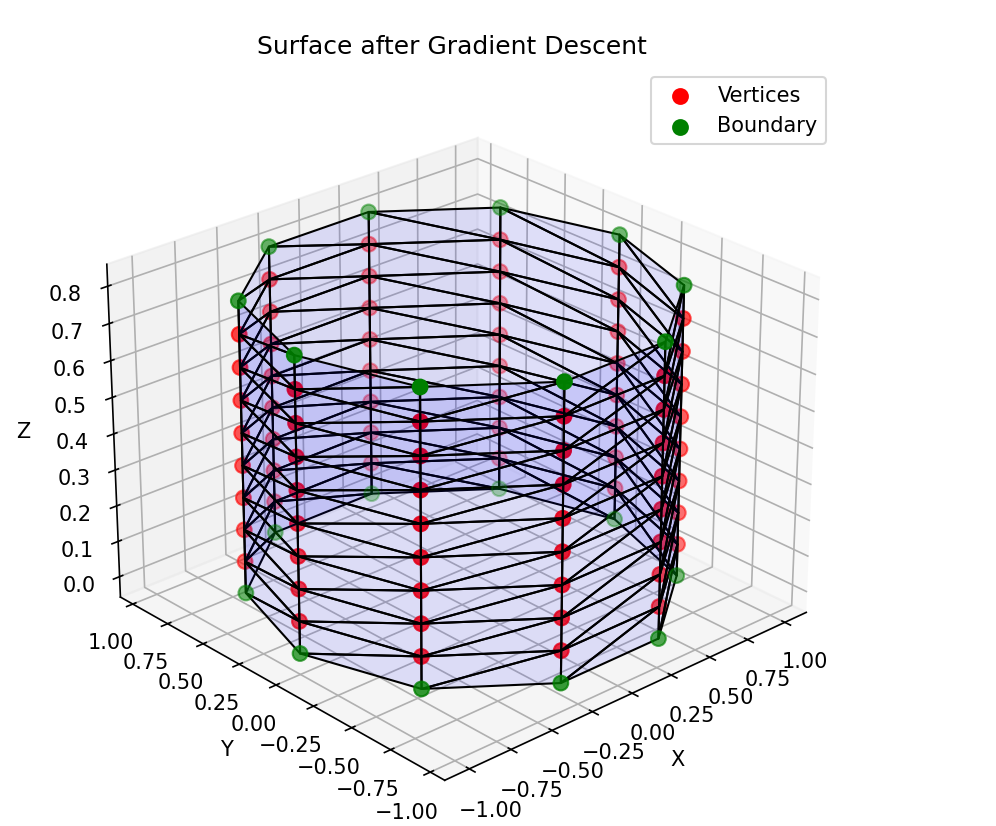
\includegraphics[width=\linewidth]{figures/img1.png}
    \caption{Triangulated mesh of a cylinder before gradient descent evolution.}
    \label{fig:ac-gd-a}
  \end{subfigure}\hfill
  \begin{subfigure}{0.49\textwidth}
    \centering
    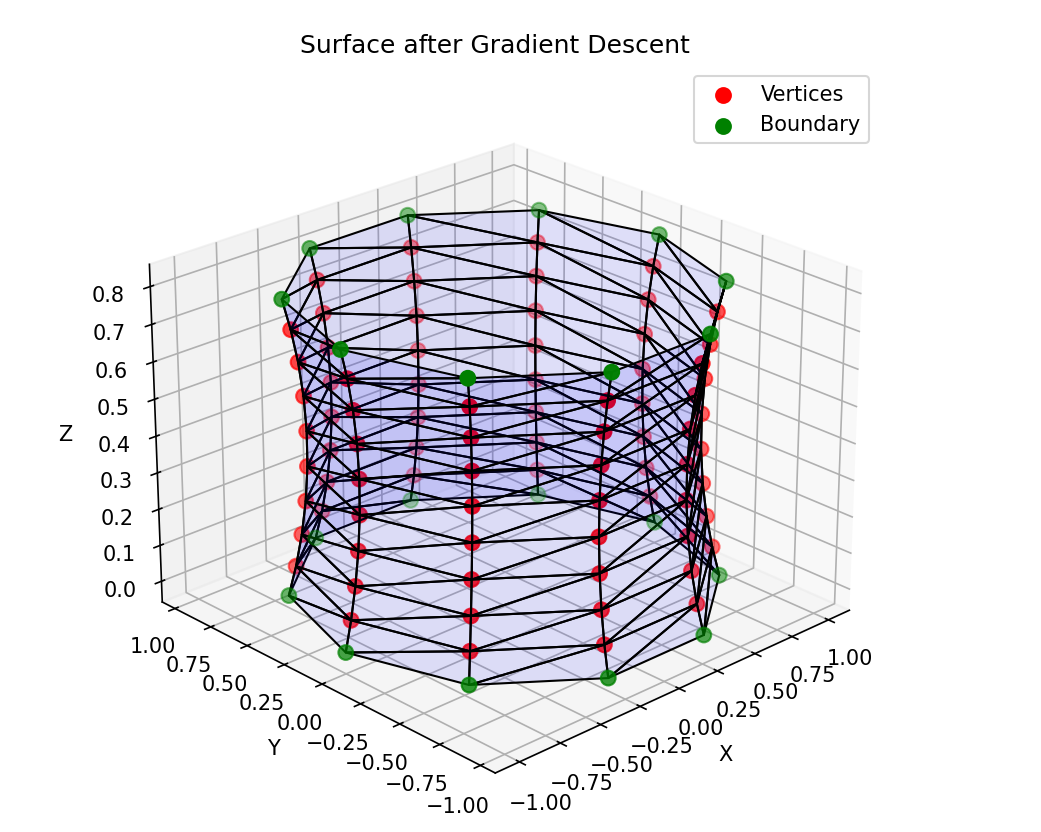
\includegraphics[width=\linewidth]{figures/img2.png}
    \caption{Evolved surface that has converged to a stable catenoid.}
    \label{fig:ac-gd-b}
  \end{subfigure}
  \caption{Minimal surface produced by FEM-based gradient descent of the discrete area functional, starting from a triangulated cylindrical mesh (left). The final configuration illustrates convergence to a stable minimal surface under the given boundary constraints (right).}
  \label{fig:ac-gd-side-by-side}
\end{figure}
\FloatBarrier
\noindent This framework provides the foundation for computing unstable minimal surfaces via the mountain–pass algorithm, and for adapting the same approach to the Allen–Cahn energy in the next subsection. And, as previously mentioned, my supervisor then implemented a comprehensive version of this application for finding unstable minimal surfaces. The algorithm behind this is outlined below.

\noindent\textbf{Mountain–pass search for unstable minimal surfaces.}\\
To find index--1 saddles of $\mathcal{A}$:
\begin{enumerate}
    \item Choose two low–area configurations $V^-$ and $V^+$ in different basins.
    \item Interpolate vertex positions to get a path $\gamma(t)$.
    \item Find $t^\star$ maximising $\mathcal{A}(\gamma(t))$.
    \item Perform gradient descent orthogonal to the path tangent at $t^\star$.
    \item Update the path and repeat until the peak energy converges.
\end{enumerate}

\noindent\textbf{Implementation notes}
\begin{itemize}
    \item \textbf{Precomputation:} store face adjacencies and edge vectors for fast gradient assembly.
    \item \textbf{Boundary constraints:} fix coordinates of boundary vertices throughout iterations.
    \item \textbf{Contributions:} I implemented the program for finding minimal surfaces and my supervisor implemented a comprehensive program for also finding unstable minimal surfaces.
\end{itemize}

\subsection{Finite Element Method for the Allen--Cahn Energy}\label{sec:planar-widths-program}
Having established a finite element framework for evolving surfaces with respect to the area functional, we now turn to the Allen--Cahn energy as a tool for studying $p$–widths. In my supervisor's approach~\cite{Guaraco18}, the Allen-Cahn equation provides a PDE-based variational framework whose min--max critical points correspond, via the volume (or length in the planar case) of their zero level--set, to approximations of the $p$--widths. Our goal in this section is therefore not only to adapt the FEM framework developed earlier to this energy, but to use it as a numerical engine for approximating $p$–width–realising hypersurfaces and visualising them in triangulated domains.

\noindent To carry out the finite element discretisation of the Allen–Cahn energy, we approximate the solution $u \in H^{1}(\Omega)$ using continuous, piecewise–linear ($P_{1}$) basis functions defined over a conforming triangulation $\mathcal{T}_{h}$ of the domain. Each basis function is associated with a mesh vertex and takes the value $1$ at its own vertex and $0$ at all others, varying linearly within each element. The figure below illustrates three such basis functions on the reference triangle, which together span the space $P_{1}(T)$ for a single element.

\begin{figure}[ht]
    \centering
    \begin{subfigure}{0.32\textwidth}
        \centering
        \begin{tikzpicture}
\begin{axis}[
  view={-135}{35},
  width=5.2cm, height=5.2cm,
  xlabel={$x$}, ylabel={$y$}, zlabel={$z$},
  xmin=0, xmax=1, ymin=0, ymax=1, zmin=0, zmax=1,
  axis lines=box, tick align=outside
]
\addplot3[
  patch, patch type=triangle,
  fill=red!85, draw=black
] coordinates {
  (0,0,1)
  (0,1,0)
  (1,0,0)
};
\end{axis}
\end{tikzpicture}
 % include the first plot
        \caption{First basis function}
        \label{fig:red}
    \end{subfigure}
    \begin{subfigure}{0.32\textwidth}
        \centering
        \begin{tikzpicture}
\begin{axis}[
  view={-35}{25},
  width=5.2cm, height=5.2cm,
  xlabel={$x$}, ylabel={$y$}, zlabel={$z$},
  xmin=0, xmax=1, ymin=0, ymax=1, zmin=0, zmax=1,
  axis lines=box, tick align=outside
]
\addplot3[
  patch, patch type=triangle,
  fill=green!80!black, draw=black
] coordinates {
  (1,0,1)
  (0,1,0)
  (0,0,0)
};
\end{axis}
\end{tikzpicture}
 % include the second plot
        \caption{Second basis function}
        \label{fig:green}
    \end{subfigure}
    \begin{subfigure}{0.32\textwidth}
        \centering
        \begin{tikzpicture}
\begin{axis}[
  view={-35}{25},
  width=5.2cm, height=5.2cm,
  xlabel={$x$}, ylabel={$y$}, zlabel={$z$},
  xmin=0, xmax=1, ymin=0, ymax=1, zmin=0, zmax=1,
  axis lines=box, tick align=outside
]
\addplot3[
  patch, patch type=triangle,
  fill=blue!85, draw=black
] coordinates {
  (1,0,0)
  (0,1,1)
  (0,0,0)
};
\end{axis}
\end{tikzpicture}
 % include the third plot
        \caption{Third basis function}
        \label{fig:blue}
    \end{subfigure}
    \caption{The three triangular basis functions plotted on the reference element.}
    \label{fig:three-basis}
\end{figure}

\noindent With these basis functions $\{\phi_i\}_{i=1}^N$ defined, we can express the finite element approximation $u_h$ of $u$ as a linear combination of them,
\[
u_{h}(x) = \sum_{i=1}^{N} U_{i} \, \phi_{i}(x), \qquad \phi_{i}|_{T} \in P_{1}(T), \quad T \in \mathcal{T}_{h}.
\]
\noindent To evaluate the energy efficiently, we work element--wise - both for clarity of formulation and to enable vectorised assembly. On each triangle \(\Delta = \mathrm{conv}\{x_{1},x_{2},x_{3}\}\) we use barycentric coordinates \(\lambda_{1},\lambda_{2},\lambda_{3}\), so that
\[
u_{h}|_{\Delta} = \sum_{a=1}^{3} u_{a} \, \lambda_{a}, \quad u_{a} := u_{h}(x_{a}).
\]
\noindent We now substitute this local representation into the Allen–Cahn energy functional, which naturally separates into a Dirichlet term and a potential term,
\begin{align*}
    E_{\varepsilon}(u) = \underbrace{\frac{\varepsilon}{2} \int_{\Omega} |\nabla u|^{2}\,\mathrm{d}x}_{\text{Dirichlet Energy}} +  \underbrace{\frac{1}{4 \varepsilon} \int_{\Omega} (1-u^2)^2 \,\mathrm{d}x.}_{\text{Potential Energy}}
\end{align*}
\textbf{Dirichlet energy term.}
Since each barycentric coordinate \(\lambda_a\) is affine on \(\Delta\), its gradient \(\nabla \lambda_a\) is constant over the element. Therefore, for $u_h|_{\Delta}$ we have
\[
\nabla u_{h}|_{\Delta} = \sum_{a=1}^{3} u_{a} \, \nabla\lambda_{a} \quad \text{(constant on $\Delta$)}.
\]
The contribution of the Dirichlet term on \(\Delta\) is then
\[
\mathrm{DE}_{\varepsilon}^{\Delta}(u_{h})
= \frac{\varepsilon}{2} \, \mathrm{Area}(\Delta) \, \Big|\sum_{a=1}^{3} u_{a} \, \nabla\lambda_{a}\Big|^{2}
= \frac{\varepsilon}{2} \, U_{\Delta}^{\top} K_{\Delta} \, U_{\Delta},
\]
where $K_{\Delta}$ is the $3\times 3$ local stiffness matrix with entries
\[
(K_{\Delta})_{ab} := \mathrm{Area}(\Delta) \, \nabla\lambda_{a} \cdot \nabla\lambda_{b}.
\]
This element–wise formulation is well suited to vectorised assembly as the constant gradients \(\nabla \lambda_a\) can be precomputed once per element 
and reused across all evaluations on \(\Delta\), avoiding redundant computation.

\noindent\textbf{Potential energy term.}
The quartic term $(1-u_{h}^{2})^{2}$ is expanded in barycentric monomials $\lambda_{1}^{\alpha}\lambda_{2}^{\beta}\lambda_{3}^{\gamma}$ and integrated exactly via
\[
\int_{\Delta} \lambda_{1}^{\alpha}\lambda_{2}^{\beta}\lambda_{3}^{\gamma} \, dx
= \frac{\alpha! \, \beta! \, \gamma!}{(\alpha+\beta+\gamma+2)!} \, 2\,\mathrm{Area}(\Delta).
\]
This yields a closed--form quartic polynomial $Q(u_{1},u_{2},u_{3})$ such that
\[
\mathrm{PE}_{\varepsilon}^{\Delta}(u_{h})
= \frac{\mathrm{Area}(\Delta)}{4\varepsilon} \ Q(u_{1},u_{2},u_{3}),
\]
The required barycentric moments up to degree~4 are precomputed and stored, so that evaluating \(Q\) and its derivatives during assembly reduces to only a handful of fused multiply--add operations per element, which are well suited to vectorised computation. This precomputation enables the element--wise contributions to be assembled rapidly in practice - an essential feature for maintaining responsiveness in the interactive application. The complete table of precomputed barycentric integrals is given in Table (\ref{appendix-3:int-table}) and the explicit form of $Q$ is provided in Equation~\eqref{eq-Q}.

\noindent\textbf{Global assembly.}
Summing over all elements,
\[
E_{\varepsilon}^{h}(U)
= \sum_{\Delta \in \mathcal{T}_{h}}
\left[ \frac{\varepsilon}{2} \, U_{\Delta}^{\top} K_{\Delta} U_{\Delta}
+ \frac{\mathrm{Area}(\Delta)}{4\varepsilon} \, Q(U_{\Delta}) \right],
\]
with exactness for $P_{1}$ shape functions. Gradients and Hessians follow by differentiating in the same way as was done in the minimal surfaces code and assembling into global vectors/matrices.


\noindent\textbf{Constrained mountain--pass search.}
To target an index--$p$ saddle, we restrict $u_{h}$ to the span of the first $p$ Dirichlet--Laplacian eigenfunctions $\{\psi_{1},\dots,\psi_{p}\}$.  
Sampling $m$ quasi--uniform points on the projective sphere $\mathbb{RP}^{p-1}$ gives initial sweep--out states
\[
U^{(j)} = \sum_{i=1}^{p} r^{(j)}_{i} \, \psi_{i}, \qquad r^{(j)} \in \mathbb{S}^{p-1}, \quad r^{(j)} \sim \text{quasi--uniform}.
\]

\noindent The algorithm is as follows:
\begin{enumerate}
    \item Initialise: Populate $\{U^{(j)}\}$ and compute $E_{\varepsilon}^{h}(U^{(j)})$.
    \item Repeat until convergence:
    \begin{enumerate}
        \item Identify $j^{\star} = \arg\max_{j} E_{\varepsilon}^{h}(U^{(j)})$.
        \item Gradient descent step:
        \[
        V \gets U^{(j^{\star})} - \alpha \, \nabla E_{\varepsilon}^{h}(U^{(j^{\star})}),
        \]
        with $\alpha$ chosen by backtracking.
        \item Project $V$ onto $\mathrm{span}\{\psi_{1},\dots,\psi_{p}\}$ and normalise to $\mathbb{RP}^{p-1}$.
        \item Replace $U^{(j^{\star})} \gets V$; optionally reparametrise to equalise $L^{2}$ arc--length between samples.
    \end{enumerate}
\end{enumerate}

\noindent\textbf{Output and index check.}
The final $U^{(j^{\star})}$ approximates an index--$p$ saddle of $E_{\varepsilon}$.  
The Morse index is estimated from the discrete Hessian
\[
H_{h} = \varepsilon K - \frac{1}{\varepsilon} M[W''(u_{h})],
\]
by counting its negative eigenvalues.

\noindent\textbf{Implementation Notes.}

\begin{itemize}
    \item \textbf{Precomputation and reuse:} For each triangle, store 
    \(\mathrm{Area}(\Delta)\), \(\nabla \lambda_a\), the barycentric moments, and the 
    local stiffness matrix \(K_\Delta\).  
    This enables vectorised evaluation across all elements without recomputation, 
    reducing memory access and floating–point operations.

    \item \textbf{Vectorised gradient assembly:} The polynomial \(Q\) and its gradient 
    \(\nabla Q\) are evaluated using precomputed barycentric integrals via table lookups, 
    allowing all elements to be processed in a single vectorised pass using only a few 
    fused multiply–add operations per element.

    \item \textbf{Sparse Hessian assembly:} FEM connectivity implies \(H_{ij} \neq 0\) only 
    if vertices \(i\) and \(j\) share an element.  
    A custom neighbour–based Hessian assembly exploits this sparsity, reducing complexity 
    from \(\mathcal{O}(N^3)\) (dense autodiff) to \(\mathcal{O}(N^2)\).
\end{itemize}

\noindent\textbf{Illustrative outputs.}
The figures below present example outputs from the interactive application developed by my supervisor, illustrating zero--level sets of functions evolved via the constrained mountain--pass search. 
The image on the left shows the zero--level set of an eigenfunction of the Laplacian operator as an initial state of the algorithm. 
The image on the right shows the evolved zero--level set, now close to realising the first width of the triangle

\begin{figure}[ht]
  \centering
  \begin{subfigure}{0.49\textwidth}
    \centering
    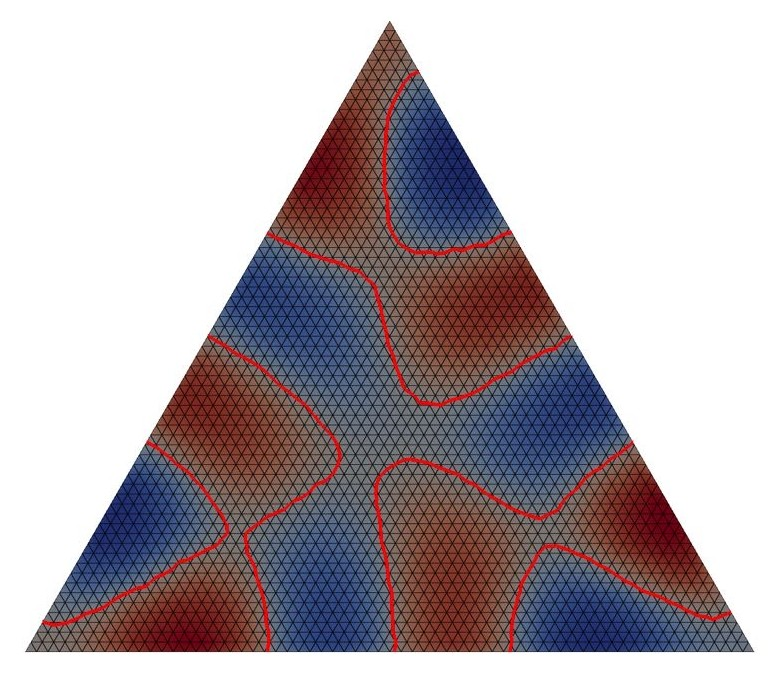
\includegraphics[width=\linewidth]{figures/width2.JPG}
    \caption{Initial state of the constrained mountain--pass search.}
  \end{subfigure}\hfill
  \begin{subfigure}{0.47\textwidth}
    \centering
    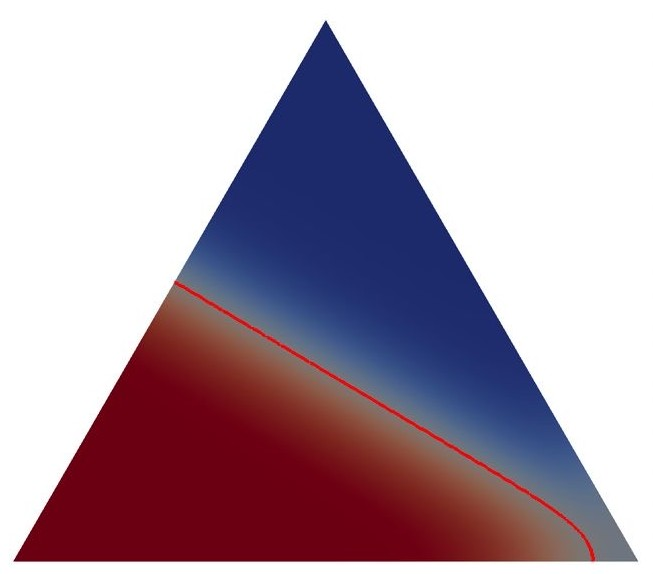
\includegraphics[width=\linewidth]{figures/width1.JPG}
    \caption{Evolved state, zero--level set close to realising the first width.}
  \end{subfigure}
  \caption{Outputs from the interactive application developed by my supervisor. The panels display the zero--level set (red curve) of a function at two successive stages of its evolution via the constrained mountain--pass search on a triangular domain, approaching the first width (right).}
\end{figure}
\FloatBarrier

\noindent Overall, the numerical framework developed here turns Guaraco’s Allen–Cahn theory into a 
practical tool for computing and visualising $p$–width–realising hypersurfaces, thereby 
linking the variational results of Chapter~\ref{ch:3} to concrete computational tests and 
conjecture verification.


\chapter{Further Directions}
\label{ch:5}

\section{Known Results for Widths}
Even for very simple planar regions, higher $p$–widths are largely unknown. Beyond a few examples there is no closed form for $\omega_p(\Omega)$:
\begin{itemize}
  \item For convex regions $\Omega\subset\mathbb{R}^2$ ,
        \begin{align*}
        \omega_1(\Omega)=\inf_{\|v\|=1}\left(\max_{x\in\Omega} x\!\cdot v-\min_{x\in\Omega} x\!\cdot v\right)
        \quad\text{(Chodosh--Cholsaipant~\cite{Chodosh25}, Chapter~\ref{ch:3}).}
        \end{align*}
    \item For the equilateral triangle inscribed in the unit disc $T\subset\mathbb{R}^2$,
        \[
        \omega_2(T)=\tfrac{3}{2}, \omega_3(T)=\tfrac{3\sqrt{3}}{2}, \omega_4(T)=3, 
        \quad\text{(Chodosh--Cholsaipant~\cite{Chodosh25}).}
        \]
  \item For the round 2-sphere $(S^2,g_0)$,
        \begin{align*}
        \omega_p(S^2,g_0)=2\pi\,\big\lfloor\sqrt{p}\,\big\rfloor
        \qquad\text{(Chodosh--Mantoulidis~\cite{Chodosh23}).}
        \end{align*}
  \item For the round projective plane $(\mathbb{RP}^2,g_0)$,
        \begin{align*}
        \omega_p(\mathbb{RP}^2,g_0)=2\pi\,\big\lfloor\tfrac{1}{4}\big(1+\sqrt{1+8p}\big)\,\big\rfloor
        \qquad\text{(Marx--Kuo~\cite{Marx-Kuo25}).}
        \end{align*}
  \item For a compact Riemannian manifold of dimension $n+1$ with metric $g$, $(M^{n+1}, g)$,
        \begin{align*}
        \omega_p(M,g) \sim\ a(n)\operatorname{Vol}_g(M)^{\frac{n}{n+1}}p^{\frac{1}{n+1}},\quad\text{as $p\to\infty,$}\qquad\text{(Liokumovich--Marques--Neves~\cite{Liokumovich18}).} 
        \end{align*}
        with a universal constant $a(n)>0$ for each $n$.  In particular, in the planar case $n=1$, we have that for regions $\Omega\subset\mathbb{R}^2$,
        \begin{align*}
        \omega_p(\Omega) \sim\ a(1)\mathrm{Area}(\Omega)^{\frac{1}{2}}p^{\frac{1}{2}},\quad \text{as $p\to\infty$.}
        \end{align*}
\end{itemize}

\section{Challenges and Opportunities in Proving Width Conjectures}

Understanding and proving explicit formulas for $p$--widths in higher dimensions remains a challenging open problem. The obstacles are structural as well as technical and arise even for geometrically simple domains.

\noindent A first challenge is that a hypersurface realising a given $p$–width need not be connected - it may consist of multiple disjoint components whose combined volume attains the width. This multiplicity phenomenon is difficult to capture in a purely variational argument and complicates any min--max characterisation, as one must control the interaction between components and ensure that the correct total measure is realised.

\noindent A second challenge lies in encoding the boundary data of slices in higher--dimensional sweep--outs.  In the planar setting, the endpoint map produces a simple $S^1 \times S^1$ parameter space, but in higher dimensions the analogous parameter space $X$ can be far more intricate. Constructing such an $X$ so that it captures all relevant boundary configurations, while remaining tractable for topological arguments, is a significant obstacle. Tracking how hypersurface boundaries split, merge, or change topology adds another layer of difficulty.

\noindent With these difficulties in mind, we cautiously conjecture for a Euclidean $d$–simplex, that the first width is equal to the minimal altitude:
\begin{conjecture}[First width of a $d$–simplex]\label{conjecture1}
Let $\Delta^d\subset\mathbb{R}^d$ be a Euclidean $d$–simplex with vertices 
$v_0,\dots,v_d$ and let 
$F_i=\operatorname{conv}\big(\{v_0,\dots,v_d\}\setminus\{v_i\}\big)$ 
be the $(d-1)$–simplex opposite $v_i$. Then
\[
  \omega_1(\Delta^d) = \min_{i=0,\dots,d}\operatorname{dist}\big(v_i,\operatorname{aff}(F_i)\big).
\]
Equivalently,
\[
  \omega_1(\Delta^d) = \min_{i=0,\dots,d}\frac{d\,\operatorname{Vol}_d(\Delta^d)}{\operatorname{Vol}_{d-1}(F_i)},
\]
since 
$\operatorname{Vol}_d(\Delta^d)
 =\tfrac{1}{d}\operatorname{Vol}_{d-1}(F_i)\cdot 
  \operatorname{dist}(v_i,\operatorname{aff}(F_i))$.
\end{conjecture}

\noindent The proof strategy outlined in Chapter~\ref{ch:3} suggests a path forward via intersection theory in an appropriate parameter space $X$, but the difficulties noted above - particularly the possibility of disconnected minimising hypersurfaces - must be addressed for this approach to succeed. One possible discretisation approach is to represent the boundary of a hypersurface in the sweep--out by a mesh of $n$ equally spaced points, mapping these to a point in $\oplus_{i=1}^d S^{d-1}$ (which in the planar case $d=2$ gives the torus $T^2 = \oplus_{i=1}^2 S^1$). As in Lemma (\ref{lem:polygon-width-ub}), one could then search for target sets that any such path must intersect to obtain upper bounds for first widths of higher–dimensional domains and potentially for higher $p$–widths.

\noindent A complementary direction for future work is provided by the numerical framework developed in Chapter~\ref{ch:4}. FEM implementations of the Allen–Cahn equation - or alternative discretisations - can be used to search for $p$--width realising hypersurfaces in a wide range of domains, including higher–dimensional simplices. By analysing the zero level sets, one can directly investigate the two key challenges above: detecting multiplicity phenomena and studying topology changes. This allows one to identify geometric features that any analytic proof must address. Such computational experiments can supply evidence for or against conjectured width formulas, guide the refinement of proof strategies, and help prioritise conjectures that are most promising for rigorous resolution.





\appendix
\chapter{Supporting Material for Chapter 1}

\section{Singular Homology Preliminaries}\label{MorseTheoryAppendix}
\begin{definition}[Standard $m$-simplex] \label{def:std-simplex}
The standard $m$--simplex is the compact set
$$ \Delta^{m}\;=\;\bigl\{(t_1,\dots,t_m)\in\mathbb R^{m}\,\big|\,t_i\ge 0,\;\sum_{i=1}^{m} t_i \le 1\bigr\}.$$ 
For $m=1$, this corresponds to the unit interval $[0,1]$.\\
For $m=2$, this corresponds to the right angled triangle with corners $(0,0), (1,0), (0,1)$.
\end{definition}

\begin{definition}[Singular $m$--chains]
Fix a coefficient ring (usually a field) $k$ and a topological space $X$.
\begin{itemize}
\item A singular $m$--simplex in $X$ is a continuous map
      $\sigma:\Delta^{m}\longrightarrow X$, where $\Delta^{m}$ is the standard
      $m$–simplex (Definition~\ref{def:std-simplex}). Intuitively for say $m=2$, this is the function which sends the 2-$d$ simplex to a crumpled triangle in the manifold $X$.

\item The free $k$–module generated by all singular $m$–simplices is
      written
      \[C_{m}(X;k):= \Bigl\{\sum_{i=1}^{\ell} a_{i}\,\sigma_{i}\;\Bigm|\;a_{i}\in k,\;\sigma_{i}:\Delta^{m}\to X\text{ singular $m$–simplices},\;\ell<\infty\Bigr\}.\]
      The sum is purely algebraic and so distinct $m$-simplices form orthogonal directions in this vector space. An element of $C_{m}(X;k)$ is called a singular $m$--chain. 
      The sum is finite, so every chain is a formal linear combination
      of only finitely many simplices.

\item The boundary operator
      $\partial_m:C_{m}(X;k)\longrightarrow C_{m-1}(X;k)$ is defined on
      a simplex by the alternating face formula
      \begin{equation}\label{boundaryOperator}
          \partial_m \sigma
        =\sum_{j=0}^{m}(-1)^{j}\,
          \sigma\!\bigl|_{[v_0,\dots,\widehat{v_j},\dots,v_m]},
      \end{equation}
      and this extends to a singular $m$-chain by summing the resulting $m-1$-simplices in the ring $k$ over the $m$-simplices in the original chain.  This results in,
      $\partial_{m-1}\circ\partial_m=0$.

\item The sequence
      \(
        \cdots\;\xrightarrow{\partial_{m+1}} C_{m}(X;k)
                \;\xrightarrow{\partial_{m}}   C_{m-1}(X;k)
                \xrightarrow{\partial_{m-1}}\;\cdots
      \)
      is the singular chain complex of $X$ with coefficients in $k$.
\end{itemize}
\end{definition}
\begin{remark}[Intuition for the alternating signs]
For a $2$–simplex (triangle embedded in $\mathbb{R}^2$) with ordered vertices $(v_0,v_1,v_2)$
the boundary formula
\[
\partial_2\sigma
  =\;
    \sigma|_{[v_1,v_2]}
  \;-\;
    \sigma|_{[v_0,v_2]}
  \;+\;
    \sigma|_{[v_0,v_1]}
\]
takes three oriented edges with signs
$+\, -\, +$.
Starting at $v_0$ this moves counter-clockwise once around the
triangle: first along $[v_1,v_2]$, then back along $[v_2,v_0]$ (hence the
minus sign), and finally along $[v_0,v_1]$.
Thus $\partial_2\sigma$ is the “loop” that encloses the triangle.

The alternating signs are chosen precisely so that when you take the
boundary again every edge appears twice with opposite orientation,
hence $\partial_{1}\!\bigl(\partial_{2}\sigma\bigr)=0$.
The same idea works in all dimensions: faces of a simplex come in
cancelling pairs, so $\partial_{m-1}\circ\partial_{m}=0$.
\end{remark}


\begin{definition}[Simplicial Complex]
Let \(V\) be a finite vertex set. A \emph{simplicial complex} \(\mathcal{K}\) on \(V\) is a collection of subsets of \(V\) such that:
\begin{enumerate}
    \item \textbf{Closed under taking faces:} If \(\sigma \in \mathcal{K}\) and \(\tau \subseteq \sigma\), then \(\tau \in \mathcal{K}\).
    \item \textbf{Contains singletons:} For every vertex \(v \in V\), the singleton \(\{v\} \in \mathcal{K}\).
\end{enumerate}
The elements of \(\mathcal{K}\) are called \emph{simplices}, and the dimension of a simplex \(\sigma\) is defined as \(\dim(\sigma) = |\sigma| - 1\), where \(|\sigma|\) is the number of elements in \(\sigma\). A \(k\)-simplex is a simplex of dimension \(k\), and the collection of all simplices of dimension at most \(k\) forms the \(k\)-skeleton of the simplicial complex.
\end{definition}


\begin{definition}[Orientation]
    Let $\sigma=[v_0,\dots,v_m]$ be an $m$–simplex with vertex set $\{v_0,\dots,v_m\}$. Two orderings of the vertices determine the same orientation iff they differ by an even permutation.
    Replacing the ordering by an odd permutation reverses the orientation. Hence an orientation of $\sigma$ is an equivalence class of orderings modulo even permutations.\\
    An orientation of a finite simplicial complex $K$ is a choice of orientation for every simplex such that the induced orientations on any common face agree, i.e.\ differ by an even permutation.
    With this choice, the boundary operator
        \[
          \partial_m[v_0,\dots,v_m]
          \;=\;\sum_{j=0}^{m}(-1)^{j}\,[v_0,\dots,\widehat{v_j},\dots,v_m]
        \]
        satisfies $\partial_{m-1}\circ\partial_m=0$ for chains over
        $\mathbb Z$.
\end{definition}

\begin{example}[A 2-boundary in the Tetrahedron]
Consider the tetrahedron $\Delta^3$ with ordered vertices $V = (v_0,v_1,v_2,v_3)$ and face set of singular $2$-simplices, $F = \{ \sigma_{012}, \sigma_{013}, \sigma_{023}, \sigma_{123} \}$, embedded in $\mathbb{R}^3$. Let us consider a chain in the free $\mathbb{Z}$-module on $\Delta^3$ generated by singular $2$-simplices, namely $C_{2}(\Delta^3;\mathbb{Z})$, which is the set of finite formal linear combinations of singular $2$-simplices. An example of such a chain is,
$$c = \sigma_{123} - \sigma_{023} + \sigma_{013} - \sigma_{012} \in C_{2}(\Delta^3;\mathbb{Z}).$$
In the alternating face formula for the boundary operator, Equation (\ref{boundaryOperator}), we have that
\begin{align*}
\partial_3 \big(\Delta^3\big) = \partial_3 (\sigma_{0123}) = \sum_{j=0}^{3}(-1)^{j}\,\sigma\!\bigl|_{[v_0,\dots,\widehat{v_j},\dots,v_4]} &= \sigma_{123} - \sigma_{023} + \sigma_{013} - \sigma_{012} = c.
\end{align*}
However, because consecutive boundary operators compose to zero ($\partial_{m-1}\circ \partial_{m}=0$) we have $$0=\partial_2(\partial_3 (\sigma_{0123})) = \partial_2 (c).$$ Hence  $c \in Z_2(\Delta^3;\mathbb{Z})$ i.e. is a $2$-cycle for $\Delta^3$.

Intuitively, an m-chain is an oriented sum of “m-dimensional edges” (simplices). The sign records which way we traverse that face: reversing the vertex order multiplies the simplex by -1. Since $c$ is a $2$-cycle its boundary vanishes meaning that every oriented 1-simplex occurs equally
often with positive and negative orientation, so when adding them “tip to tail” they cancel out and the chain starts where it ended, thus we have the name “cycle”.

\noindent We can in fact say more, $c$ is not only a cycle but also a boundary. Indeed, $$\partial_3 \big(\Delta^3\big) = c.$$
As stated in Definition (\ref{cycles_n_boundaries}), from an algebraic viewpoint a boundary is an $m$-chain that lies in the image of the boundary operator; geometrically, however, it is an $m$-cycle that \emph{exactly bounds} some $(m+1)$-simplex (here the 3-simplex \(\sigma_{0123}\)).  Every boundary is therefore a cycle (\(\partial_{m-1}\!\circ\partial_{m}=0\)), but not every cycle is a
boundary: a cycle may “loop around a hole” without enclosing any higher-dimensional simplex.
\end{example}

\begin{remark}
For a path-connected topological manifold $X$, the $0$-th order Homology group for $X$, $H_0(X;k)$, is isomorphic to $k$. This is because the set of $0$ chains, $C_0(X;k)$, is simply all finite formal linear combinations of points in $X$ with coefficients in $k$ and the set of $0$-cycles is all $0$-chains due to $0$-simplices having no boundary. $B_0 = im(\partial_1)$ is the subgroup of $C_0$ that is generated by the set of formal differences of points that have a path passing through both (endpoints of an oriented 1-simplex), which is the set of formal linear combinations of points in $X$ with the sum of coefficients, $0$ according to addition in $k$. Two $0$-chains, $c_1$ and $c_2$, are thus in the same equivalence class under $\sim_0$ iff they have the same total sum of coefficients and so the equivalence classes are just the possible totals, namely $k$.
\end{remark}

\begin{lemma}\label{lem:A1}
For topological space $X$ and a coefficient field $k$, the Homology groups $H_m(X;k)$ are vector spaces.
\end{lemma}
\begin{proof}
The Chain groups $C_m(X;k)$ from a vector space over $k$ as they inherit coefficient addition form a field and they are just finite formal linear combinations of $m$-simplices - the set of distinct singular $m$-simplices form the basis.

By definition, the map $\partial_m:C_{m}(X;k)\longrightarrow C_{m-1}(X;k)$ is linear over singular $m$-simplices. Thus, $Z_m = \ker(\partial_m)$ and $B_m=\operatorname{im}(\partial_{m+1})$ are linear subspaces of $C_m(X;k)$.

Now if $V$ is a vector space and $W\leq V$ a subspace, the quotient $V/W$ inherits addition and scalar multiplication from V; hence it is again a vector space over the same field $k$. Taking $V=Z_m$ and $W=B_m$, the result follows.
\end{proof}
\chapter{Supporting Material for Chapter 2}\label{appendix-2}
\section{Geometry}
\begin{definition}[Diffeomorphism]
Let $V$ and $M$ be two differentiable manifolds and $f:V\to M$ be a map between them. We say that $f$ is a \emph{diffeomorphism} if both $f$ and its inverse map $f^{-1}$ are continuously differentiable. If $f(V) = M$, we say that $V$ and $M$ are diffeomorphic. 
\end{definition}

\noindent From the definition it is immediate that the inverse of a diffeomorphism is a diffeomorphism and that compositions of diffeomorphisms are one, too. The composition of diffeomorphisms is associative as they are functions and the identity map is a diffeomorphism; hence, the set of diffeomorphisms on a manifold have a group structure.

\begin{definition}[Diffeomorphism Group]
Let $M$ be a smooth (infinitely differentiable) manifold that is second-countable and Hausdorff. The group $\operatorname{Diff}(M)$ is the set of smooth diffeomorphisms on $M$, with composition.
\end{definition}

\begin{definition}[Homotopy]
Let $X$ and $Y$ be two topological spaces and $f_0, f_1:X\to Y$ both be continuous. A \emph{homotopy} is a continuous function $H: [0,1]\times X \to Y$ such that $H(0,x)=f_0(x)$ and $H(1,x)=f_1(x)$, in which case we say that $f_0$ and $f_1$ are homotopic.
\end{definition}

\begin{remark}[$\operatorname{Diff}_0(M)$]
The set of smooth diffeomorphisms  $\operatorname{Diff}_0(M)$, homotopic to the identity, is a subgroup of $\operatorname{Diff}(M)$
\end{remark}

\begin{definition}[Immersion]
An \emph{immersion} is a differentiable function $f:V \to M$ between differentiable manifolds such that the differential, $d_pf: T_pV \to T_{f(p)}M$, is injective at every $p\in M$.
\end{definition}

\begin{definition}[Embedding]
The smooth map $f:V\to M$ is said to be an \emph{embedding} if:
\begin{enumerate}
    \item It is an immersion i.e. its derivative is everywhere injective.
    \item $f$ is a homeomorphism of $V$ onto its image $f(V)$.
\end{enumerate}
\end{definition}

\begin{definition}[Isotopy]\label{def:isotopy}
 Let $V$ and $M$ be two differentiable manifolds and $f_0, f_1 : X\to Y$ both be smooth. An \emph{Isotopy} is a continuous function $F: [0,1]\times V \to M$ such that for each $t\in [0,1]$, the map $F(t,x) =: F_t(x):V\to M$ is an embedding.
\end{definition}

\begin{remark}\label{remark:embediffdiff}
It can be shown by the Constant Rank Theorem that $f$ being an embedding is equivalent to it being a smooth map whose image is diffeomorphic to its domain (\ref{lem:embediffdiff}).
\end{remark}

\begin{lemma}\label{lem:embediffdiff}
Let $f:V\to M$ be a smooth map between differentiable manifolds that is immersive and a homeomorphism of $V$ onto its image $f(V)$ then $f$ is a diffeomorphism between $V$ and $f(V)$.
\end{lemma}
\begin{proof}
For $f$ to be an immersion it is necessary that $k := \dim V \leq \dim M =: n$. Let $y_0 = f(v_0) \in f(V)$ be some fixed point. By the Constant Rank Theorem there exists smooth functions (with well-defined and smooth inverses)
$$\varphi_1:U\subset V \to \mathbb{R}^k \quad \text{and} \quad \varphi_2:N\subset M \to \mathbb{R}^n$$ 
such that 
\begin{equation}\label{eq:charts}
\varphi_2\big(f\big(\varphi_1^{-1}(u_1,\cdots,u_k)\big)\big) = (u_1,\cdots,u_k,0,\cdots,0).
\end{equation}
Restricting $\varphi_2(N)$ to the subspace of $M$, $M_0$ where the last $n-k$ coordinates are $0$, we have that $\varphi_2^{-1}(M_0) = N \cap f(V)$. 
Since $f$ is a homeomorphism of $V$ onto is image it is bijective onto its image and so the inverse $\big(f|_{U} \big)^{-1}:f(U)\to U$ is well defined and bijective. Expressing this inverse using Equation (\ref{eq:charts}),
$$\big(f|_{U} \big)^{-1} = \varphi_1^{-1} \circ \pi \circ \varphi_2,$$
where $\pi:\mathbb{R}^k \times \mathbb{R}^{n-k} \to \mathbb{R}^k, \pi\big(\vec{u},\vec{0}\big) = \vec{u}$. Since $\pi$ is a projection it is smooth, thus the whole map is a composition of smooth maps and so $\big(f|_{U} \big)^{-1}$ is smooth.\\
For each $v \in V$ the $U_v$ guaranteed by the Constant Rank Theorem produces images $f(U_v)$. The union of these images covers $f(V)$ and so we can apply the above construction for each $v$, to produce a smooth map onto $f(V)$. Note this map agrees on different $U_v$ that may overlap due to $f$ being injective. We can glue these maps together, giving a smooth global inverse $f^{-1}:f(V)\to V$, thus $f$ is a diffeomorphism of $V$ onto its image.
\end{proof}

\begin{definition}[Degree]
If $\sigma: S^1\to S^1$ then the induced group homomorphism $\sigma_*:H_1(S^1)\cong \mathbb{Z} \to H_1(S^1)\cong \mathbb{Z}$ is multiplication by a unique integer $a$, because $\mathbb{Z}$ is the free abelian group on one generator. Define $\operatorname{deg}(\sigma)=a$.
\end{definition}

\noindent\textbf{Equivalent formulation of Winding Number \cite{stein03}.}
If $f$ is $C^1$ and $z_0\in\Omega$, writing $\gamma(\theta):=f(e^{i\theta})$,
\[
\operatorname{wind}(f)=\frac{1}{2\pi} \big(\Delta\arg\!\big(\gamma(\theta)-z_0\big) \pmod{2\pi}\big)
=\frac{1}{2\pi i}\int_0^{2\pi}\frac{\gamma'(\theta)}{\gamma(\theta)-z_0}\,d\theta.
\]

\begin{definition}[Degree in Higher Dimensions]\label{def:deg-higher-dims}
If $\sigma: \partial\Delta^d \cong S^{d-1}\to \partial\Delta^d\cong S^{d-1}$ then the induced group homomorphism $\sigma_*:H_{d-1}(S^{d-1})\cong \mathbb{Z} \to H_{d-1}(S^{d-1})\cong \mathbb{Z}$ is still multiplication by a unique integer $a$. Define $\operatorname{deg}(\sigma)=a$.
\end{definition}



\chapter{Supporting Material for Chapter 3}

\section{Table of Precomputed Integrals and Polynomials} \label{appendix-3:int-table}

\renewcommand{\arraystretch}{1.2} % global, tidy spacing
\begin{align}
\begin{array}{c|c|c}
\text{monomial} & \int_{\Delta_i}\text{(monomial)}\,dx & \text{name} \\ \hline
\lambda_i & \tfrac{1}{3}  & I_{100} \\
\lambda_i^2 & \tfrac{1}{6} & I_{200} \\
\lambda_i\lambda_j & \tfrac{1}{12} & I_{110} \\
\lambda_i^3 & \tfrac{1}{10} & I_{300} \\
\lambda_i^2\lambda_j & \tfrac{1}{30} & I_{210} \\
\lambda_1\lambda_2\lambda_3 & \tfrac{1}{60} & I_{111} \\
\lambda_i^4 & \tfrac{1}{15} & I_{400} \\
\lambda_i^3\lambda_j & \tfrac{1}{60} & I_{310} \\
\lambda_i^2\lambda_j^2 & \tfrac{1}{90} & I_{220} \\
\lambda_i^2\lambda_j\lambda_k & \tfrac{1}{180} & I_{211} \\
\end{array}
\end{align}

\begin{align}\label{eq-Q}
Q(u_1, u_2, u_3) 
= 1 & + I_{400}(u_1^4+u_2^4+u_3^4) -  2I_{200}(u_1^2+u_2^2+u_3^2)  \nonumber \\
& -4I_{110}(u_1u_2 + u_1u_3+u_2u_3) + 6I_{220}(u_1^2u_2^2 + u_1^2u_3^2+u_2^2u_3^2) \nonumber \\
& +4I_{310}(u_1u_2^3 + u_1^3u_2 + u_1u_3^3+ u_1^3u_3 + u_2u_3^3 + u_2^3u_3) \nonumber \\
& +12I_{211}(u_1^2u_2u_3 + u_1u_2^2u_3 + u_1u_2u_3^2)
\end{align}





%%%%%%%%%%%%%%%%%%%%%%%%%%%%%%%%%%%%%
\bibliography{bibliography.bib}
%%%%%%%%%%%%%%%%%%%%%%%%%%%%%%%%%%%%%

\end{document}